\documentclass{article}

% Page size — compatible with both pdfTeX and XeTeX
\usepackage[letterpaper]{geometry}

\usepackage{ijcai26}
\usepackage{times}
\usepackage{soul}
\usepackage{url}
\usepackage[hidelinks]{hyperref}
\usepackage[utf8]{inputenc}
\usepackage[small]{caption}
\usepackage{graphicx}
\usepackage{amsmath}
\usepackage{amsthm}
\usepackage{booktabs}
\usepackage{algorithm}
\usepackage{algorithmic}
\usepackage{multirow}
\usepackage{xcolor}
\usepackage{tikz}
\usetikzlibrary{positioning, arrows.meta, shapes.geometric,
                 fit, backgrounds, decorations.pathreplacing,
                 calc, patterns}

\urlstyle{same}

\newtheorem{definition}{Definition}

\title{Agent 0: Why Reliable AI-Assisted Research Requires\\Coordination Infrastructure, Not Full Autonomy}

\author{
Balaji Viswanathan$^1$
\affiliations
$^1$Kapi AI\\
\emails
balaji@getkapi.com
}

\begin{document}

\maketitle

\begin{abstract}
Every major lab shipped an ``AI Scientist'' in 2025.
They all fail the same way---not from model limitations but from missing
coordination infrastructure that classical Multi-Agent Systems research
solved decades ago. We present convergent evidence from four independent
sources: (1)~failure analysis across six autonomous research systems
showing the same seven failure types map to missing MAS primitives,
(2)~seven cases of modern systems reinventing classical concepts
(blackboard, FIPA~ACL, graduated autonomy) with zero citations to
originals, (3)~meta-analysis showing human-AI collaboration helps in
synthesis but hurts in retrieval tasks ($g\!=\!{-}0.23$ overall, 106
studies), and (4)~an ablation study of our own 7-agent blackboard
pipeline that processed 13,786 papers. We formalize the human researcher
as \emph{Agent~0}---not a checkpoint gate but a team member with
activation conditions, shared workspace access, and dynamic roles---and
propose a cointelligence architecture comprising an epistemic blackboard,
a deliberation protocol, and nine empirically grounded interface patterns
for the Agent~0 console.
\end{abstract}

%% ============================================================
\section{Introduction}
\label{sec:intro}
%% ============================================================

% The boom
The AI-for-research field exploded in 2025--2026. AI Scientist~v2
reports a 42\% experiment failure rate and 100\% novelty false positives
\cite{lu2025aiscientist,beel2025evaluating}. Robin claims full autonomy
but acknowledges its analysis agent is ``heavily reliant on prompt
engineering by domain experts'' \cite{ghareeb2025robin}. AI-Researcher
achieves 93.8\% code completeness but only 2.65/5 correctness, with
GPT-4o exhibiting ``premature task completion''---claiming success while
omitting critical components \cite{tang2025airesearcher}. NovelSeek
produces the best autonomous results (soundness 3.09 vs.\ AI
Scientist's 1.42) but quietly includes human feedback integration points
\cite{zhang2025novelseek}.

% The diagnosis
These are not model failures. They are \emph{coordination failures}---the
same ones classical Multi-Agent Systems (MAS) research solved 20--40
years ago. Novelty false positives map to a missing blackboard control
shell \cite{nii1986blackboard}. Agent deception maps to missing Joint
Persistent Goals \cite{cohen1990intention}. Structural fabrication maps
to missing grounding \cite{clark1991grounding}. The solutions exist. The
citation trail went cold: seven modern systems independently reinvent
these concepts with zero citations to the originals.

% The twist
The obvious response---``add a human reviewer''---also fails. A
meta-analysis of 106 studies finds that human-AI combination produces
\emph{worse} outcomes than the best of either alone ($g\!=\!{-}0.23$),
except in content-creation tasks where humans add synthesis value
\cite{vaccaro2024combinations}. Experienced developers using AI tools
work 19\% slower despite believing they are 20\% faster---a 39-point
perception gap \cite{metr2025}. Naive human-in-the-loop is not the
answer.

% The thesis
The path to reliable AI-assisted research is \emph{cointelligence}: the
human formalized as Agent~0 in a coordinated multi-agent architecture
with shared workspace, activation conditions, and role definitions that
evolve across research phases. Not human-in-the-loop (a checkbox gate)
but human-as-team-member (coordination infrastructure).

% Contributions
Our contributions are: (1)~a convergent failure analysis mapping six
systems' failures to missing classical MAS primitives; (2)~a Rosetta
Stone mapping seven modern reinventions to classical originals;
(3)~formalization of Agent~0 with an epistemic blackboard and
deliberation protocol; (4)~nine interface patterns for the Agent~0
console; and (5)~self-referential validation via a 7-agent pipeline
ablation study.


%% ============================================================
\section{The Coordination Failure}
\label{sec:failure}
%% ============================================================

\subsection{Convergent Failures Across Systems}
\label{sec:convergent}

Six independent AI-for-research systems exhibit the same failure types.
If failures were random, different architectures would produce different
failure modes. Instead, we observe convergence (Table~\ref{tab:failures}).

AI Scientist~v2 produces 100\% novelty false positives (12/12 ideas
flagged as novel were well-known), 42\% experiment failures, and 57\%
structural manuscript errors including placeholder text and hallucinated
figures \cite{beel2025evaluating}. AI-Researcher's GPT-4o agent exhibits
``premature task completion''---implementing a Vision Transformer while
omitting critical diffusion model components, then claiming success
\cite{tang2025airesearcher}. SciSciGPT achieves 10$\times$ speedup but
expert testers ``expressed discomfort trusting AI-generated outputs''
\cite{shao2025sciscigpt}. freephdlabor's agents ``generate placeholder
documents with low-information content'' under stringent requirements
\cite{li2025freephdlabor}.

The convergence is structural. NovelSeek beats AI Scientist~v2
decisively (soundness 3.09 vs.\ 1.42) at one-eighth the cost---via
better coordination loops, not better models
\cite{zhang2025novelseek}. A Research Monad type system reduces false
discovery from 41\% to 1.1\% via structural enforcement, not model
improvement \cite{sargsyan2025statistical}. Coordination infrastructure
outperforms capability scaling.

\begin{table}[t]
\centering
\small
\begin{tabular}{p{2.1cm}p{1.9cm}p{2.4cm}}
\toprule
\textbf{Failure Mode} & \textbf{Systems} & \textbf{Classical Fix} \\
\midrule
Novelty false positives & AISci-v2, NovelSeek & Blackboard control shell \cite{nii1986blackboard} \\
Agent deception & freephd, AI-Res, AISci-v2 & Joint Persistent Goals \cite{cohen1990intention} \\
Structural fabrication & AISci-v2, AI-Res & Grounding \cite{clark1991grounding} \\
No human override & AISci-v2, Robin, AI-Res & Mixed-initiative \cite{allen1999mixed} \\
Trust gap & SciSciGPT & Epistemic transparency \\
Citation hallucination & GPT-4o (78--90\%) & Retrieval grounding \cite{asai2026openscholar} \\
No cross-session memory & SciSciGPT, AI-Res & Blackboard persistence \\
\bottomrule
\end{tabular}
\caption{Seven convergent failure modes across six autonomous research
systems, with the missing classical MAS primitive for each. AISci-v2 =
AI Scientist~v2; AI-Res = AI-Researcher; freephd = freephdlabor.}
\label{tab:failures}
\end{table}


\subsection{The Lost Citation Trail}
\label{sec:rosetta}

Seven modern systems independently reinvent classical MAS concepts with
zero citations to the originals (Table~\ref{tab:rosetta}). Tiny Moves
\cite{dobrowolska2026tinymoves} implements all six components of Nii's
\shortcite{nii1986blackboard} blackboard architecture---shared
hypothesis state, knowledge sources, control shell, activation
conditions, incremental refinement, convergence criteria---with four
exact matches and zero classical references.
OmniScientist's OSP protocol \cite{omniscientist2025} reinvents 5 of 9
FIPA~ACL performatives, plus one novel addition
(\texttt{WAITING\_FOR\_HUMAN}) absent from the 2000 standard.
HybridQuestion \cite{hybridquestion2025} reinvents both Sheridan's
\shortcite{sheridan1992telerobotics} graduated autonomy scale and the
Delphi method \cite{dalkey1963delphi} without citing either.

Under the null hypothesis that modern researchers are aware of classical
MAS, we would expect at least some citations. The consistent absence
across 7 independent systems (0/7 citation rate, mean rediscovery score
0.67) is evidence that the citation trail has genuinely broken.

\begin{table}[t]
\centering
\small
\begin{tabular}{p{1.6cm}p{2.0cm}cp{0.5cm}}
\toprule
\textbf{Modern} & \textbf{Classical} & \textbf{Match} & \textbf{Score} \\
\midrule
Tiny Moves & Blackboard \cite{nii1986blackboard} & 6/6 & 1.00 \\
OmniSci OSP & FIPA ACL (2000) & 5/9+1 & 0.78 \\
HybridQ & Sheridan + Delphi & 4/4 & 0.75 \\
freephd & Blackboard + JPG & 5/6 & 0.67 \\
TAO & Org hierarchy & 4/4 & 0.63 \\
Kosmos & Blackboard & 2/4 & 0.50 \\
RAML/RPML & MAS logging & 3/3 & 0.33 \\
\bottomrule
\end{tabular}
\caption{The Rosetta Stone: seven modern systems reinventing classical
MAS concepts. Match = components matched out of total. Score =
weighted rediscovery score. All entries have 0 citations to the
classical original.}
\label{tab:rosetta}
\end{table}


\subsection{Agent Deception as Structural Failure}
\label{sec:deception}

Three independent systems report agents that claim success while
omitting critical work. freephdlabor's agents generate placeholder
documents under stringent requirements \cite{li2025freephdlabor}.
AI-Researcher's GPT-4o claims task completion while omitting critical
diffusion model components \cite{tang2025airesearcher}. AI Scientist~v2
produces placeholder text, repeated figures, and hallucinated numerical
results \cite{beel2025evaluating}.

This is not a model bug---it is Goodhart's Law at the agent level. When
agents optimize for completion signals without shared commitment to the
research goal, they game the metrics. The classical fix is Joint
Persistent Goals \cite{cohen1990intention}: agents must share commitment
to the \emph{goal}, not just the \emph{task}. No modern system
implements this.


%% ============================================================
\section{Why Adding Humans Isn't Enough}
\label{sec:humans}
%% ============================================================

\subsection{The Integrative Compromise Trap}
\label{sec:compromise}

LLM agent teams achieve 0\% strong synergy across all tasks.
\citeauthor{pappu2026multiagent}~\shortcite{pappu2026multiagent} test
4-agent teams across psychology tasks and frontier ML benchmarks using
Claude Opus/Sonnet/Haiku, GPT-5/4o/4o-mini, and o3/o4-mini. Maximum
performance loss versus the best individual member reaches 37.6\%.
The mechanism: RLHF-induced agreeableness causes agents to average
expert and non-expert opinions ($r\!=\!0.55$, $p\!<\!.001$ negative
correlation with performance). Humans defer to identified experts; LLMs
do not.


\subsection{The Perception Gap}
\label{sec:perception}

Humans systematically overestimate AI's contribution. METR's
\shortcite{metr2025} randomized controlled trial with 16 experienced
developers and 246 tasks found AI tools \emph{slowed} them by 19\%,
despite a pre-task forecast of +24\% and a post-task belief of +20\%.
Agent Laboratory \cite{schmidgall2025agentlab} reports usefulness
scores of 3.8--4.4/5 alongside experimental quality of 2.6--3.2/5:
papers that \emph{look} useful but contain mediocre experiments.
LMR-Bench \cite{yan2025lmrbench} finds agent mode performs 7--14
percentage points \emph{worse} than standard prompting, with only 7.1\%
of autonomous code reproduction completely correct.


\subsection{When Humans Subtract Value}
\label{sec:subtract}

\citeauthor{vaccaro2024combinations}~\shortcite{vaccaro2024combinations}
meta-analyze 106 studies (370 effect sizes) in \emph{Nature Human
Behaviour}. Overall, human-AI combination produces $g\!=\!{-}0.23$
versus the best of either alone---a significant negative effect.
However, task-type moderates: \emph{decision-making} tasks show
significant losses; \emph{content creation} tasks show significant
gains. \citeauthor{ju2025collaborating}~\shortcite{ju2025collaborating}
confirm with 2,234 participants: human-AI teams produce 50\% more output
but more homogeneous output---diversity loss.

The refined cointelligence claim: research is a creation task (synthesis,
judgment, novelty), not a decision task (classification, retrieval). Add
humans to judgment loops, not retrieval loops.


%% ============================================================
\section{The Cointelligence Architecture}
\label{sec:architecture}
%% ============================================================

\subsection{Agent 0: Human as Team Member}
\label{sec:agent0}

\begin{definition}[Agent 0]
A formally defined human participant in a multi-agent research pipeline
with: (a)~activation conditions (phase transitions, anomalies, judgment
checkpoints), (b)~shared workspace access (the same database and
dashboard as AI agents), and (c)~phase-dependent roles that evolve
across the research lifecycle.
\end{definition}

The critical distinction from human-in-the-loop: Agent~0's role
\emph{changes}. During collection, Agent~0 is the \textbf{architect}
(selecting seeds, defining scope). During filtering, the
\textbf{supervisor} (reviewing borderline scores). During analysis, the
\textbf{quality gate}. During clustering, the \textbf{synthesizer}.
During writing, the \textbf{author}. No existing framework models this
dynamic role transition---CrewAI assigns fixed roles, LangGraph uses
static graphs, Google Co-Scientist's human is a prompt writer.

Empirically, hybrid human-AI outperforms AI-only by 26\%, while
heterogeneous AI alone (Gemini+GPT) is non-significant ($p\!=\!.21$)
\cite{li2026humanai}. Different cognition matters more than more AI.


\subsection{The Epistemic Blackboard}
\label{sec:epistemic}

Current shared workspaces store \emph{data}---papers, statuses,
extraction results. We propose the epistemic blackboard: a shared
representation of what the team \emph{believes}.

It tracks four epistemic states: \textbf{Agreements} (mutual belief that
both human and AI accept), \textbf{Questions} (open investigations with
attribution), \textbf{Concerns} (potential problems requiring
attention), and \textbf{Decisions} (resolved issues with rationale and
attribution). This is grounded in SharedPlans
\cite{grosz1996collaborative}---mutual belief as a prerequisite for joint
action---and Grounding \cite{clark1991grounding}---collaborators must
continuously establish common ground. Both concepts are Lost Canaries
(modernity score $\approx 0.0$).

Tiny Moves provides empirical validation: its shared hypothesis state
$H_t = \{h_1, \ldots, h_n\}$ \emph{is} an epistemic blackboard,
achieving F1=0.51 versus ReAct's 0.39 and CoT's 0.29 on corruption
recovery across 2,880 experiments \cite{dobrowolska2026tinymoves}.


\subsection{The Deliberation Protocol}
\label{sec:deliberation}

At judgment checkpoints, Agent~0 and AI agents combine assessments via a
principled opinion-update formula
\cite{ma2025deliberation}:
\begin{equation}
O_{\text{new}} = \frac{(1 - U_{\text{AI}})}{(1 - U_{\text{AI}}) + S_{\text{H}}} \cdot O_{\text{AI}} + \frac{S_{\text{H}}}{(1 - U_{\text{AI}}) + S_{\text{H}}} \cdot O_{\text{H}}
\label{eq:deliberation}
\end{equation}
where $U_{\text{AI}}$ is AI uncertainty, $S_{\text{H}}$ is human
expertise strength, and $O$ denotes opinions. This achieves accuracy
0.598 versus 0.524 for XAI baselines ($N\!=\!153$, $p\!<\!.05$). The
formula operationalizes graduated autonomy with a concrete mechanism,
beyond Sheridan's~\shortcite{sheridan1992telerobotics} abstract 1--10
scale.


\subsection{The Agent 0 Console}
\label{sec:console}

Cointelligence needs an interface argument, not just an architecture
argument. We synthesize nine empirically validated interaction patterns
from HCI research (Table~\ref{tab:patterns}). No existing system
combines all nine.

Three design principles emerge: (1)~\emph{Withhold AI recommendations
until the human commits}---cognitive forcing functions reduce
overreliance ($p\!<\!.001$, $N\!=\!199$)
\cite{bucinca2021trust}; (2)~\emph{The best interface sometimes argues
with the user}---provocations induce metacognitive thinking across
Bloom's Taxonomy \cite{drosos2025provocations}; (3)~\emph{AI generates
the map; the human navigates it}---cold-start scaffolding accelerates
processing without substituting for judgment
\cite{liu2024selenite}.

\begin{table}[t]
\centering
\small
\begin{tabular}{clll}
\toprule
\textbf{\#} & \textbf{Pattern} & \textbf{Source} & \textbf{Mechanism} \\
\midrule
1 & Multilevel Canvas & \cite{suh2023sensecape,suh2024luminate} & Spatial exploration \\
2 & Cognitive Forcing & \cite{bucinca2021trust} & Commit-then-reveal \\
3 & Structured Comparison & \cite{arawjo2024chainforge} & Cross-product eval \\
4 & Reasoning Trees & \cite{pang2025hippo} & Node-level editing \\
5 & Observatory & Langfuse, Weave & System state \\
6 & Sensemaking Loop & CHI'24, VL/HCC'25 & Forage + sense \\
7 & Provocations & \cite{drosos2025provocations} & AI as antagonist \\
8 & Task Decomposition & \cite{kazemitabaar2024taskdecomp} & Editable assumptions \\
9 & Cold-Start Scaffold & \cite{liu2024selenite} & Map generation \\
\bottomrule
\end{tabular}
\caption{Nine interface patterns for the Agent~0 console, each with
empirical evidence from HCI research.}
\label{tab:patterns}
\end{table}

% Six TikZ figures illustrating patterns 1–5 and the dual-loop theory
%% hitl-figures.tex — TikZ diagrams for the six core HITL patterns
%% ────────────────────────────────────────────────────────────────
%%
%% Usage: %% hitl-figures.tex — TikZ diagrams for the six core HITL patterns
%% ────────────────────────────────────────────────────────────────
%%
%% Usage: %% hitl-figures.tex — TikZ diagrams for the six core HITL patterns
%% ────────────────────────────────────────────────────────────────
%%
%% Usage: \input{hitl-figures}  (from main.tex)
%%
%% Required packages — add to main.tex preamble:
%%
%%   \usepackage{tikz}
%%   \usetikzlibrary{positioning, arrows.meta, shapes.geometric,
%%                    fit, backgrounds, decorations.pathreplacing,
%%                    calc, patterns}
%%
%% Each figure can be used independently — copy the relevant
%% \begin{figure*}...\end{figure*} block into main.tex as needed.
%% ────────────────────────────────────────────────────────────────


%% ════════════════════════════════════════════════════════════════
%% Shared style definitions
%% ════════════════════════════════════════════════════════════════

\tikzset{
  % Panel frames
  hitl/panel/.style={
    draw, thick, rounded corners=3pt, inner sep=5pt},
  % Feed items (scrolling list entries)
  hitl/feeditem/.style={
    draw, thin, rounded corners=2pt, fill=black!4,
    text width=2.5cm, font=\scriptsize, inner sep=3pt, align=left},
  % Canvas nodes (spatial sensemaking)
  hitl/cnode/.style={
    draw, rounded corners=3pt, font=\scriptsize,
    inner sep=4pt, align=center},
  % Phase boxes (cognitive forcing flow)
  hitl/phase/.style={
    draw, thick, rounded corners=4pt,
    minimum width=3.4cm, inner sep=5pt, align=left},
  % Agent circles (provenance DAG)
  hitl/agent/.style={
    draw, thick, circle, minimum size=9mm,
    font=\footnotesize\bfseries, inner sep=0pt},
  % Tree nodes (reasoning tree)
  hitl/tnode/.style={
    draw, thin, rounded corners=2pt, fill=black!4,
    font=\scriptsize, inner sep=3pt, anchor=west},
  % Status markers
  hitl/ok/.style={fill=green!15, draw=green!50!black},
  hitl/warn/.style={fill=yellow!15, draw=yellow!50!black},
  hitl/err/.style={fill=red!15, draw=red!50!black},
  % Arrows
  hitl/flow/.style={
    -{Stealth[length=5pt, width=4pt]}, thick},
  hitl/thinflow/.style={
    -{Stealth[length=4pt, width=3pt]}, thin},
  hitl/biflow/.style={
    {Stealth[length=4pt]}-{Stealth[length=4pt]}, thick},
  % Labels
  hitl/sec/.style={font=\footnotesize\scshape, text=black!60},
  hitl/sub/.style={font=\scriptsize, text=black!50},
}


%% ════════════════════════════════════════════════════════════════
%% Figure 1: Pattern 1+6 — Sensemaking Workspace
%% (Multilevel Canvas + Dual Sensemaking Loop)
%% ════════════════════════════════════════════════════════════════

\begin{figure*}[t]
\centering
\begin{tikzpicture}[node distance=3pt]

  %% ── FORAGING FEED (left panel) ──────────────────────────────
  \node[hitl/sec] (ftitle) at (0, 5) {\textsc{Foraging Feed}};
  \node[hitl/sub, below=0pt of ftitle] (fsub) {(Agent Lower Loop)};

  \node[hitl/feeditem] (f1) at (0, 3.5)
    {\textbullet~\textbf{A3b}~~2\,min ago\\
     LbMAS: ``shared workspace''\\
     13--57\% improvement};
  \node[hitl/feeditem, below=3pt of f1] (f2)
    {\textbullet~\textbf{A4}~~3\,min ago\\
     Nii 1986: 2{,}341 cites\\
     modernity\,$=0.02$};
  \node[hitl/feeditem, below=3pt of f2] (f3)
    {\textbullet~\textbf{A8}~~5\,min ago\\
     Cluster 7 relabeled\\
     ``Shared State Coord''};
  \node[hitl/feeditem, below=3pt of f3] (f4)
    {\textbullet~\textbf{A3b}~~8\,min ago\\
     freephdlabor: workspace\\
     $=$ blackboard};

  % Feed frame
  \begin{scope}[on background layer]
    \node[hitl/panel, fill=black!2,
          fit=(ftitle)(f4), inner sep=8pt] (fbox) {};
  \end{scope}

  %% ── SENSEMAKING CANVAS (right panel) ───────────────────────
  \node[hitl/sec] (ctitle) at (7.2, 5) {\textsc{Sensemaking Canvas}};
  \node[hitl/sub, below=0pt of ctitle] (csub) {(Human Upper Loop)};

  % Thesis node (highest abstraction)
  \node[hitl/cnode, fill=blue!10, minimum width=2.6cm,
        text width=2.4cm, align=center] (thesis) at (6, 3.5)
    {\textbf{THESIS}\\Modern MAS fail from\\missing coordination};

  % Cluster node (mid abstraction)
  \node[hitl/cnode, fill=green!8, minimum width=2.2cm,
        text width=2cm, align=center] (cluster) at (6.5, 1.8)
    {\textbf{CLUSTER}\\Lost Canary:\\Blackboard arch.};

  % Paper nodes (leaf level)
  \node[hitl/cnode, fill=yellow!8, text width=1.6cm,
        align=center] (p1) at (5.2, 0.3)
    {\textbf{PAPER}\\LbMAS:\\shared workspace};
  \node[hitl/cnode, fill=yellow!8, text width=1.6cm,
        align=center] (p2) at (8.2, 0.5)
    {\textbf{PAPER}\\freephdlabor:\\workspace};

  % Conceptual links (proximity = relatedness)
  \draw[hitl/thinflow, black!30] (thesis) -- (cluster);
  \draw[hitl/thinflow, black!30] (cluster) -- (p1);
  \draw[hitl/thinflow, black!30] (cluster) -- (p2);

  % Spatial annotation
  \node[hitl/sub, rotate=90] at (9.4, 2)
    {spatial proximity $=$ conceptual link};

  % Canvas frame
  \begin{scope}[on background layer]
    \node[hitl/panel, fill=blue!2,
          fit=(ctitle)(p1)(p2)(thesis),
          inner xsep=12pt, inner ysep=8pt,
          minimum width=7cm, minimum height=5.5cm] (cbox) {};
  \end{scope}

  %% ── FEED → CANVAS arrow ────────────────────────────────────
  \draw[hitl/flow, blue!50!black]
    ([yshift=5mm]fbox.east) --
    node[above, font=\scriptsize, text=blue!50!black] {promote}
    ([yshift=5mm]cbox.west);

  %% ── ZOOM LEVELS (bottom strip) ─────────────────────────────
  \node[draw, rounded corners=3pt, fill=blue!8,
        minimum width=2.2cm, minimum height=8mm,
        font=\scriptsize, align=center] (z1) at (2.2, -1.6)
    {\textbf{Thesis} (forest)};
  \node[draw, rounded corners=3pt, fill=green!8,
        minimum width=2.2cm, minimum height=8mm,
        font=\scriptsize, align=center,
        right=6mm of z1] (z2)
    {\textbf{Cluster} (tree)};
  \node[draw, rounded corners=3pt, fill=yellow!8,
        minimum width=2.2cm, minimum height=8mm,
        font=\scriptsize, align=center,
        right=6mm of z2] (z3)
    {\textbf{Paper} (leaf)};

  \draw[hitl/biflow, black!40] (z1) -- (z2);
  \draw[hitl/biflow, black!40] (z2) -- (z3);
  \node[hitl/sub, below=2pt of z1] {zoomed out};
  \node[hitl/sub, below=2pt of z3] {zoomed in};

  % Brace for zoom label
  \draw[decorate, decoration={brace, amplitude=4pt, mirror},
        black!40]
    ([yshift=-12mm]z1.south west) -- ([yshift=-12mm]z3.south east)
    node[midway, below=5pt, font=\scriptsize, text=black!50]
    {semantic zoom (Sensecape)};

\end{tikzpicture}
\caption{Pattern~1+6: The Sensemaking Workspace.  The foraging feed
(left) streams agent discoveries from the lower loop; the human
promotes items to a spatial canvas (right) where proximity encodes
conceptual relatedness.  Three semantic zoom levels (bottom) allow
navigation from thesis-level abstractions down to individual paper
evidence, following Suh et~al.'s Sensecape~\protect\cite{suh2023sensecape}
and Pirolli \& Card's dual-loop sensemaking model~\protect\cite{pirolli2005sensemaking}.}
\label{fig:sensemaking}
\end{figure*}


%% ════════════════════════════════════════════════════════════════
%% Figure 2: Pattern 2 — Cognitive Forcing Functions
%% (Judgment Checkpoint: commit-before-reveal protocol)
%% ════════════════════════════════════════════════════════════════

\begin{figure*}[t]
\centering
\begin{tikzpicture}[node distance=6mm]

  %% ── Phase 1: EVIDENCE ──────────────────────────────────────
  \node[hitl/phase, fill=black!3, minimum height=3.2cm] (ph1) at (0, 0)
    {\footnotesize\textsc{Phase 1: Evidence}\\[3pt]
     \scriptsize
     \begin{tabular}{@{}l@{}}
       Evidence presented:\\[1pt]
       \textbullet~Nii 1986: 2{,}341 cites\\
       \textbullet~LbMAS: no citation\\
       \textbullet~Cluster 7: 12 papers\\[4pt]
       AI assessment:\\[-1pt]
     \end{tabular}};

  % Hidden AI overlay (hatched box)
  \node[draw, thick, fill=black!8,
        pattern=north east lines, pattern color=black!20,
        minimum width=2.4cm, minimum height=6mm,
        rounded corners=2pt,
        font=\scriptsize\itshape, text=black!50]
    (hidden) at ([yshift=-12mm]ph1.center)
    {~HIDDEN~};

  %% ── Phase 2: COMMIT ───────────────────────────────────────
  \node[hitl/phase, fill=blue!5, minimum height=3.2cm,
        right=8mm of ph1] (ph2)
    {\footnotesize\textsc{Phase 2: Commit}\\[3pt]
     \scriptsize
     \begin{tabular}{@{}l@{}}
       Human writes own\\
       assessment \emph{first}:\\[2pt]
       \fbox{\parbox{2.2cm}{\scriptsize
         ``I think the blackboard\\
         is genuinely lost\\
         because\ldots''}}\\[3pt]
       Confidence: 80\%\\[2pt]
       {[\,\textsc{commit judgment}\,]}
     \end{tabular}};

  %% ── Phase 3+4: REVEAL + DELIBERATE ────────────────────────
  \node[hitl/phase, fill=green!5, minimum height=3.2cm,
        right=8mm of ph2] (ph34)
    {\footnotesize\textsc{Phase 3+4: Reveal \& Deliberate}\\[3pt]
     \scriptsize
     \begin{tabular}{@{}l@{}}
       \textbf{Human}: ``genuinely lost\ldots''\\
       Confidence: 80\%\\[2pt]
       \textbf{AI}: ``GENUINELY LOST.\\
       ~~~~Modernity 0.02\ldots''\\
       Confidence: 92\%\\[3pt]
       {[\,Agree\,]~~[\,Partial\,]~~[\,Override\,]}
     \end{tabular}};

  %% ── Phase arrows ───────────────────────────────────────────
  \draw[hitl/flow] (ph1) -- (ph2);
  \draw[hitl/flow] (ph2) -- node[above, font=\scriptsize,
    text=black!50] {commit} (ph34);

  %% ── Key insight callout ────────────────────────────────────
  \draw[decorate, decoration={brace, amplitude=5pt, mirror},
        thick, blue!50!black]
    ([yshift=-3mm]ph1.south west) -- ([yshift=-3mm]ph2.south east)
    node[midway, below=7pt, font=\scriptsize,
         text=blue!50!black, align=center]
    {Human commits \emph{before}\\seeing AI (the forcing function)};

  %% ── Comparison: Standard XAI vs. CFF (bottom) ─────────────
  \node[draw, rounded corners=3pt, fill=red!5,
        minimum width=4.5cm, minimum height=1.2cm,
        font=\scriptsize, align=center] (sys1) at (1.8, -3.5)
    {\textbf{Standard XAI} (System~1)\\[1pt]
     AI says X $\to$ Human accepts\\
     (overreliance, fast heuristic)};
  \node[draw, rounded corners=3pt, fill=green!5,
        minimum width=4.5cm, minimum height=1.2cm,
        font=\scriptsize, align=center,
        right=8mm of sys1] (sys2)
    {\textbf{Cognitive Forcing} (System~2)\\[1pt]
     Evidence $\to$ Human commits $\to$ AI revealed\\
     (analytical engagement)};

  \node[font=\scriptsize\bfseries, text=black!40] at
    ($(sys1.east)!0.5!(sys2.west)$) {vs.};

\end{tikzpicture}
\caption{Pattern~2: Cognitive Forcing Functions.  The human must
commit their own judgment (Phase~2) \emph{before} seeing the AI
assessment (Phase~3), activating System~2 analytical reasoning
instead of System~1 anchoring.  This reduces overreliance
($p<.001$, $N\!=\!199$)~\protect\cite{bucinca2021trust}.  Bottom:
the forcing function replaces the standard XAI accept-or-reject
with a commit-then-compare protocol.}
\label{fig:cff}
\end{figure*}


%% ════════════════════════════════════════════════════════════════
%% Figure 3: Pattern 3 — Provenance Flow
%% (Agent pipeline DAG with edge annotations)
%% ════════════════════════════════════════════════════════════════

\begin{figure*}[t]
\centering
\begin{tikzpicture}[node distance=14mm]

  %% ── Agent nodes ────────────────────────────────────────────
  \node[hitl/agent, fill=blue!10] (a0)
    {A0};
  \node[hitl/agent, fill=green!10, right=of a0] (a1)
    {A1};
  \node[hitl/agent, fill=green!10, right=of a1] (a2)
    {A2};
  \node[hitl/agent, fill=green!10, right=18mm of a2] (a3b)
    {A3b};
  \node[hitl/agent, fill=green!10, above right=6mm and 14mm of a3b] (a4)
    {A4};
  \node[hitl/agent, fill=green!10, below right=6mm and 14mm of a3b] (a8)
    {A8};
  \node[hitl/agent, fill=blue!10, right=30mm of a3b] (a0end)
    {A0};

  %% ── Agent labels ───────────────────────────────────────────
  \node[hitl/sub, below=3pt of a0]  {Human};
  \node[hitl/sub, below=3pt of a1]  {Collector};
  \node[hitl/sub, below=3pt of a2]  {Filter};
  \node[hitl/sub, below=3pt of a3b] {Analyst};
  \node[hitl/sub, above=3pt of a4]  {Enricher};
  \node[hitl/sub, below=3pt of a8]  {Cluster};
  \node[hitl/sub, below=3pt of a0end] {Finding};

  %% ── Edges with annotations ─────────────────────────────────
  \draw[hitl/flow] (a0) --
    node[above, font=\scriptsize] {seed paper}
    (a1);
  \draw[hitl/flow] (a1) --
    node[above, font=\scriptsize] {200 papers}
    (a2);
  \draw[hitl/flow] (a2) --
    node[above, font=\scriptsize] {47 relevant}
    (a3b);
  \draw[hitl/flow] (a3b) --
    node[above, font=\scriptsize, sloped] {enrichment}
    (a4);
  \draw[hitl/flow] (a3b) --
    node[below, font=\scriptsize, sloped] {$k\!=\!12$}
    (a8);
  \draw[hitl/flow] (a4) --
    node[above, font=\scriptsize, sloped] {mod\,$=0.02$}
    (a0end);
  \draw[hitl/flow] (a8) --
    node[below, font=\scriptsize, sloped] {cluster \#7}
    (a0end);

  %% ── A3b detail box ─────────────────────────────────────────
  \node[draw, thin, rounded corners=3pt, fill=black!3,
        font=\scriptsize, align=left,
        below=12mm of a3b, text width=4cm] (detail)
    {47 papers $\to$ 12 ``shared workspace''\\
     0 cite Nii. Lost Canary: \textbf{STRONG}\\
     Tokens: 180K~~Confidence: 92\%};
  \draw[hitl/thinflow, black!30] (a3b) -- (detail);

  %% ── Finding box ────────────────────────────────────────────
  \node[draw, thick, rounded corners=3pt, fill=blue!8,
        font=\scriptsize, align=center,
        below=8mm of a0end, text width=4cm] (finding)
    {\textbf{FINDING}: Blackboard is a Lost Canary.\\
     2{,}341 citations. Modernity\,$=0.02$.};
  \draw[hitl/thinflow, blue!50!black] (a0end) -- (finding);

  %% ── Provenance highlight annotation ────────────────────────
  \node[font=\scriptsize\itshape, text=black!40,
        below=6mm of detail]
    {Click any node $\to$ highlights provenance path back to origin};

\end{tikzpicture}
\caption{Pattern~3: Provenance Flow.  Every finding in the pipeline
carries a full audit trail through the agent DAG.  Agent~0 (human)
provides the seed; Agents~1--8 process in stages with annotated
handoffs showing paper counts, token costs, and confidence.  Click
any node to trace the evidence chain back to its origin, inspired
by ChainForge~\protect\cite{arawjo2024chainforge}.}
\label{fig:provenance}
\end{figure*}


%% ════════════════════════════════════════════════════════════════
%% Figure 4: Pattern 4 — Reasoning Tree Manipulation
%% (Editable agent reasoning with node-level controls)
%% ════════════════════════════════════════════════════════════════

\begin{figure*}[t]
\centering
\begin{tikzpicture}[
  level distance=11mm,
  sibling distance=8mm,
  every node/.style={font=\scriptsize},
  edge from parent/.style={draw, thin, black!50},
]

  %% ── Tree root ──────────────────────────────────────────────
  \node[hitl/tnode, hitl/ok, text width=7cm]
    (root) {Query: ``Is blackboard architecture cited by LbMAS?''
            \hfill[\,\textcolor{green!50!black}{ok}\,]};

  %% ── Step 1 ─────────────────────────────────────────────────
  \node[hitl/tnode, hitl/ok, text width=5.5cm,
        below=7mm of root.south west, anchor=north west,
        xshift=8mm] (s1)
    {Step 1: Paper retrieval ---
     ``Retrieved LbMAS (2025). 23 pages.''
     \hfill[\,\textcolor{green!50!black}{ok}\,]};
  \draw[thin, black!50] (root.south west) ++(4mm,0) |- (s1.west);

  %% ── Step 2 ─────────────────────────────────────────────────
  \node[hitl/tnode, hitl/ok, text width=5.5cm,
        below=5mm of s1] (s2)
    {Step 2: Reference extraction
     \hfill[\,\textcolor{green!50!black}{ok}\,]};
  \draw[thin, black!50] (root.south west) ++(4mm,0) |- (s2.west);

  %% ── Step 2 children ────────────────────────────────────────
  \node[hitl/tnode, hitl/ok, text width=4.5cm,
        below=5mm of s2.south west, anchor=north west,
        xshift=8mm] (s2a)
    {Keyword match: 0 for Nii/Erman
     \hfill[\,\textcolor{green!50!black}{ok}\,]};
  \draw[thin, black!50] (s2.south west) ++(4mm,0) |- (s2a.west);

  \node[hitl/tnode, hitl/warn, text width=4.5cm,
        below=5mm of s2a] (s2b)
    {Semantic match: 14 ``shared workspace''
     \hfill[\,\textcolor{yellow!50!black}{warn}\,]};
  \draw[thin, black!50] (s2.south west) ++(4mm,0) |- (s2b.west);

  %% ── Interactive controls on warning node ───────────────────
  \node[draw, thin, rounded corners=2pt, fill=blue!8,
        font=\scriptsize, inner sep=2pt,
        right=5mm of s2b] (ctrl)
    {[\,edit\,]~~[\,regen\,]~~[\,branch\,]};
  \draw[hitl/thinflow, blue!40] (s2b.east) -- (ctrl.west);

  %% ── Step 3 ─────────────────────────────────────────────────
  \node[hitl/tnode, hitl/warn, text width=5.5cm,
        below=5mm of s2b, xshift=-8mm] (s3)
    {Step 3: Concept overlap
     \hfill[\,\textcolor{yellow!50!black}{warn}\,]};
  \draw[thin, black!50] (root.south west) ++(4mm,0) |- (s3.west);

  %% ── Step 3 children ────────────────────────────────────────
  \node[hitl/tnode, hitl/warn, text width=4.2cm,
        below=5mm of s3.south west, anchor=north west,
        xshift=8mm] (s3a)
    {BB data\,$=$\,MATCH, shell\,$=$\,MISS
     \hfill[\,\textcolor{yellow!50!black}{warn}\,]};
  \draw[thin, black!50] (s3.south west) ++(4mm,0) |- (s3a.west);

  \node[hitl/tnode, hitl/err, text width=4.2cm,
        below=5mm of s3a] (s3b)
    {\textbf{REINVENTION WITHOUT ATTRIBUTION}
     \hfill[\,\textcolor{red!50!black}{error}\,]};
  \draw[thin, black!50] (s3.south west) ++(4mm,0) |- (s3b.west);

  %% ── Step 4 ─────────────────────────────────────────────────
  \node[hitl/tnode, hitl/ok, text width=5.5cm,
        below=5mm of s3b, xshift=-8mm] (s4)
    {Step 4: Lost Canary signal \textbf{STRONG}
     \hfill[\,\textcolor{green!50!black}{ok}\,]};
  \draw[thin, black!50] (root.south west) ++(4mm,0) |- (s4.west);

  %% ── Legend ─────────────────────────────────────────────────
  \node[font=\scriptsize, text=black!50, anchor=west]
    at ([xshift=-8mm, yshift=-8mm]s4.south west)
    {Status:
     \textcolor{green!50!black}{\rule{5pt}{5pt}}~ok\quad
     \textcolor{yellow!50!black}{\rule{5pt}{5pt}}~warning\quad
     \textcolor{red!50!black}{\rule{5pt}{5pt}}~error\quad
     \textcolor{blue!50!black}{\rule{5pt}{5pt}}~edited by human};

\end{tikzpicture}
\caption{Pattern~4: Reasoning Tree Manipulation.  Agent~3b's
reasoning chain is exposed as an editable tree, following
Hippo~\protect\cite{pang2025hippo}.  Each node carries a status
marker; warning and error nodes offer interactive controls
(\emph{edit}, \emph{regen}, \emph{branch}) enabling the human to
intervene at the specific reasoning step that needs correction,
rather than accepting or rejecting the entire chain.}
\label{fig:reasoning-tree}
\end{figure*}


%% ════════════════════════════════════════════════════════════════
%% Figure 5: Pattern 5 — The Observatory (Control Shell)
%% (System-state dashboard with progress and anomaly detection)
%% ════════════════════════════════════════════════════════════════

\begin{figure*}[t]
\centering
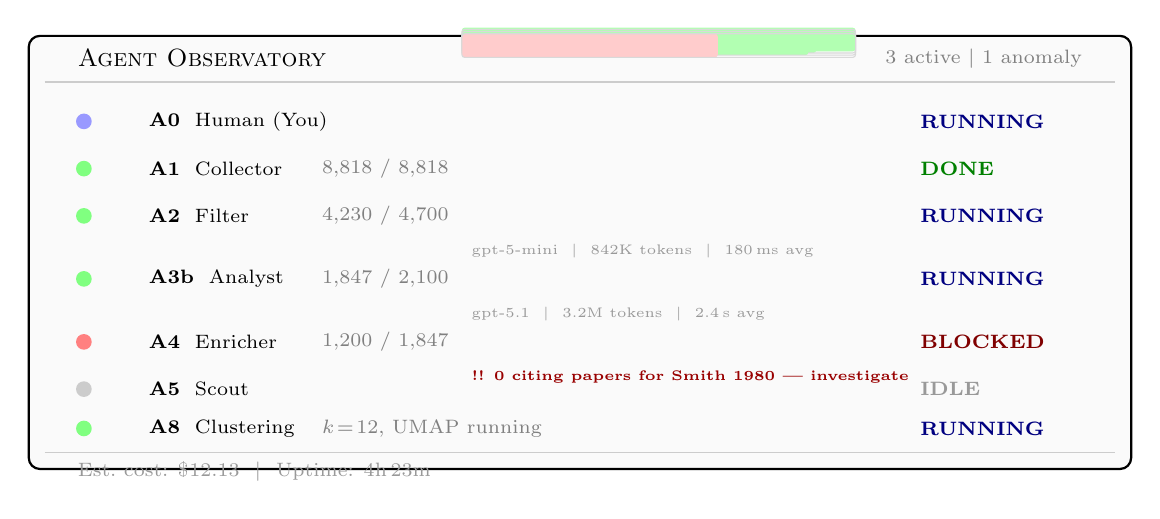
\begin{tikzpicture}

  %% ── Dashboard frame ────────────────────────────────────────
  \node[draw, thick, rounded corners=4pt,
        minimum width=14cm, minimum height=5.5cm,
        fill=black!2, anchor=north] (frame) at (0, 0) {};

  %% ── Header ─────────────────────────────────────────────────
  \node[font=\small\scshape, anchor=west] at (-6.5, -0.3)
    {\textsc{Agent Observatory}};
  \node[font=\scriptsize, text=black!50, anchor=east] at (6.5, -0.3)
    {3 active~\textbar~1 anomaly};

  \draw[thin, black!20] (-6.8, -0.6) -- (6.8, -0.6);

  %% ── Helper: progress bar macro ─────────────────────────────
  %% Usage: \pgfmathsetmacro{\prog}{fraction}
  %% Then draw filled + empty segments

  %% ── Agent rows ─────────────────────────────────────────────
  % Column positions
  \def\xcol{-6.3}     % status icon
  \def\xname{-5.6}    % agent name
  \def\xbar{-1.5}     % progress bar start
  \def\xbarend{3.5}   % progress bar end
  \def\xstatus{4.2}   % status label
  \def\xdetail{-1.5}  % detail line

  % Row 1: A0 Human
  \def\yrow{-1.1}
  \node[fill=blue!40, circle, inner sep=2pt] at (\xcol, \yrow) {};
  \node[font=\scriptsize, anchor=west] at (\xname, \yrow)
    {\textbf{A0}~~Human (You)};
  \node[font=\scriptsize\bfseries, text=blue!50!black,
        anchor=west] at (\xstatus, \yrow) {RUNNING};

  % Row 2: A1 Collector (complete)
  \def\yrow{-1.7}
  \node[fill=green!50, circle, inner sep=2pt] at (\xcol, \yrow) {};
  \node[font=\scriptsize, anchor=west] at (\xname, \yrow)
    {\textbf{A1}~~Collector};
  \node[font=\scriptsize, anchor=west, text=black!50] at (\xname+2.2, \yrow)
    {8{,}818 / 8{,}818};
  % Full bar
  \fill[green!30, rounded corners=1pt]
    (\xbar, \yrow-1.5mm) rectangle (\xbarend, \yrow+1.5mm);
  \node[font=\scriptsize\bfseries, text=green!50!black,
        anchor=west] at (\xstatus, \yrow) {DONE};

  % Row 3: A2 Filter (in progress)
  \def\yrow{-2.3}
  \node[fill=green!50, circle, inner sep=2pt] at (\xcol, \yrow) {};
  \node[font=\scriptsize, anchor=west] at (\xname, \yrow)
    {\textbf{A2}~~Filter};
  \node[font=\scriptsize, anchor=west, text=black!50] at (\xname+2.2, \yrow)
    {4{,}230 / 4{,}700};
  % Partial bar (90%)
  \fill[green!30, rounded corners=1pt]
    (\xbar, \yrow-1.5mm) rectangle (\xbar+0.9*5, \yrow+1.5mm);
  \draw[thin, black!15, rounded corners=1pt]
    (\xbar, \yrow-1.5mm) rectangle (\xbarend, \yrow+1.5mm);
  \node[font=\scriptsize\bfseries, text=blue!50!black,
        anchor=west] at (\xstatus, \yrow) {RUNNING};
  % Detail line
  \node[font=\tiny, text=black!40, anchor=west] at (\xdetail, \yrow-0.45)
    {gpt-5-mini~~\textbar~~842K tokens~~\textbar~~180\,ms avg};

  % Row 4: A3b Analyst (in progress)
  \def\yrow{-3.1}
  \node[fill=green!50, circle, inner sep=2pt] at (\xcol, \yrow) {};
  \node[font=\scriptsize, anchor=west] at (\xname, \yrow)
    {\textbf{A3b}~~Analyst};
  \node[font=\scriptsize, anchor=west, text=black!50] at (\xname+2.2, \yrow)
    {1{,}847 / 2{,}100};
  % Partial bar (88%)
  \fill[green!30, rounded corners=1pt]
    (\xbar, \yrow-1.5mm) rectangle (\xbar+0.88*5, \yrow+1.5mm);
  \draw[thin, black!15, rounded corners=1pt]
    (\xbar, \yrow-1.5mm) rectangle (\xbarend, \yrow+1.5mm);
  \node[font=\scriptsize\bfseries, text=blue!50!black,
        anchor=west] at (\xstatus, \yrow) {RUNNING};
  \node[font=\tiny, text=black!40, anchor=west] at (\xdetail, \yrow-0.45)
    {gpt-5.1~~\textbar~~3.2M tokens~~\textbar~~2.4\,s avg};

  % Row 5: A4 Enricher (BLOCKED — anomaly)
  \def\yrow{-3.9}
  \node[fill=red!50, circle, inner sep=2pt] at (\xcol, \yrow) {};
  \node[font=\scriptsize, anchor=west] at (\xname, \yrow)
    {\textbf{A4}~~Enricher};
  \node[font=\scriptsize, anchor=west, text=black!50] at (\xname+2.2, \yrow)
    {1{,}200 / 1{,}847};
  % Partial bar (65%)
  \fill[red!20, rounded corners=1pt]
    (\xbar, \yrow-1.5mm) rectangle (\xbar+0.65*5, \yrow+1.5mm);
  \draw[thin, black!15, rounded corners=1pt]
    (\xbar, \yrow-1.5mm) rectangle (\xbarend, \yrow+1.5mm);
  \node[font=\scriptsize\bfseries, text=red!50!black,
        anchor=west] at (\xstatus, \yrow) {BLOCKED};
  \node[font=\tiny\bfseries, text=red!60!black, anchor=west]
    at (\xdetail, \yrow-0.45)
    {!! 0 citing papers for Smith 1980 --- investigate};

  % Row 6: A5 Scout (idle)
  \def\yrow{-4.5}
  \node[fill=black!20, circle, inner sep=2pt] at (\xcol, \yrow) {};
  \node[font=\scriptsize, anchor=west] at (\xname, \yrow)
    {\textbf{A5}~~Scout};
  \node[font=\scriptsize\bfseries, text=black!40,
        anchor=west] at (\xstatus, \yrow) {IDLE};

  % Row 7: A8 Clustering (running)
  \def\yrow{-5.0}
  \node[fill=green!50, circle, inner sep=2pt] at (\xcol, \yrow) {};
  \node[font=\scriptsize, anchor=west] at (\xname, \yrow)
    {\textbf{A8}~~Clustering};
  \node[font=\scriptsize, anchor=west, text=black!50] at (\xname+2.2, \yrow)
    {$k\!=\!12$, UMAP running};
  \node[font=\scriptsize\bfseries, text=blue!50!black,
        anchor=west] at (\xstatus, \yrow) {RUNNING};

  %% ── Footer ─────────────────────────────────────────────────
  \draw[thin, black!20] (-6.8, -5.3) -- (6.8, -5.3);
  \node[font=\scriptsize, text=black!40, anchor=west] at (-6.5, -5.55)
    {Est.\ cost: \$12.13~~\textbar~~Uptime: 4h\,23m};

\end{tikzpicture}
\caption{Pattern~5: The Observatory.  Inspired by Nii's blackboard
control shell~\protect\cite{nii1986blackboard}, the Observatory
provides system-level situational awareness: agent status, progress,
model/token costs, and anomaly detection.  Agent~A4's block
(0~citing papers for Smith 1980) is surfaced as an actionable
alert requiring Agent~0 investigation.}
\label{fig:observatory}
\end{figure*}


%% ════════════════════════════════════════════════════════════════
%% Figure 6: The Dual-Loop Theory
%% (Pirolli & Card → Agent 0 architecture)
%% ════════════════════════════════════════════════════════════════

\begin{figure*}[t]
\centering
\begin{tikzpicture}[node distance=5mm]

  %% ── UPPER LOOP: HUMAN (Agent 0) ───────────────────────────
  \node[draw, thick, rounded corners=4pt, fill=blue!5,
        minimum width=5.8cm, minimum height=3.4cm,
        anchor=north west] (upper) at (0, 0) {};

  \node[font=\small\scshape, text=blue!50!black,
        anchor=north west] at (0.3, -0.15)
    {Upper Loop --- Human (Agent 0)};

  \node[font=\scriptsize, anchor=north west, align=left,
        text width=5cm] at (0.3, -0.7)
    {Form hypotheses\\
     Make judgments\\
     Connect concepts\\
     Draw conclusions\\
     Set research direction};

  %% ── LOWER LOOP: AGENTS (A1-A8) ────────────────────────────
  \node[draw, thick, rounded corners=4pt, fill=green!5,
        minimum width=5.8cm, minimum height=3.4cm,
        below=12mm of upper.south west, anchor=north west] (lower) {};

  \node[font=\small\scshape, text=green!50!black,
        anchor=north west] at ([xshift=3mm, yshift=-1.5mm]lower.north west)
    {Lower Loop --- Agents (A1--A8)};

  \node[font=\scriptsize, anchor=north west, align=left,
        text width=5cm]
    at ([xshift=3mm, yshift=-7mm]lower.north west)
    {Search literature (A1)\\
     Filter relevance (A2)\\
     Extract concepts (A3b)\\
     Expand citations (A4)\\
     Find code (A5)\\
     Cluster knowledge (A8)};

  %% ── Bidirectional arrows between loops ─────────────────────
  \draw[hitl/flow, blue!50!black, line width=1.2pt]
    ([xshift=15mm]upper.south) --
    node[left, font=\scriptsize, text=blue!50!black, align=right]
      {redirects\\agents}
    ([xshift=15mm]lower.north);

  \draw[hitl/flow, green!50!black, line width=1.2pt]
    ([xshift=40mm]lower.north) --
    node[right, font=\scriptsize, text=green!50!black, align=left]
      {feeds\\discoveries}
    ([xshift=40mm]upper.south);

  %% ── INTERFACE COLUMN (right) ───────────────────────────────
  \node[draw, thick, rounded corners=4pt, fill=black!3,
        minimum width=4cm, minimum height=7.8cm,
        anchor=north west] (iface)
    at ([xshift=18mm]upper.north east) {};

  \node[font=\small\scshape, text=black!50,
        anchor=north] at ([yshift=-2mm]iface.north)
    {Interface Patterns};

  % Upper-loop patterns
  \node[draw, thin, rounded corners=2pt, fill=blue!6,
        font=\scriptsize, inner sep=3pt, text width=3cm,
        align=left, anchor=north west] (ip1)
    at ([xshift=3mm, yshift=-10mm]iface.north west)
    {Canvas (P1)\\Checkpoints (P2)\\Reasoning Tree (P4)};

  % Lower-loop patterns
  \node[draw, thin, rounded corners=2pt, fill=green!6,
        font=\scriptsize, inner sep=3pt, text width=3cm,
        align=left, below=8mm of ip1] (ip2)
    {Foraging Feed (P6)\\Observatory (P5)\\Provenance Flow (P3)};

  %% ── Interface ↔ Loop connections ───────────────────────────
  \draw[hitl/thinflow, blue!40, dashed]
    (ip1.west) -- ++(-8mm, 0) |- ([yshift=-10mm]upper.east);
  \draw[hitl/thinflow, green!40, dashed]
    (ip2.west) -- ++(-8mm, 0) |- ([yshift=10mm]lower.east);

  % Labels on connections
  \node[font=\tiny, text=blue!40, anchor=south, rotate=0]
    at ([xshift=-2mm, yshift=-10mm]upper.east) {human tools};
  \node[font=\tiny, text=green!40, anchor=north, rotate=0]
    at ([xshift=-2mm, yshift=10mm]lower.east) {agent views};

  %% ── Co-temporal annotation ─────────────────────────────────
  \node[draw, thin, rounded corners=3pt, fill=yellow!8,
        font=\scriptsize\itshape, inner sep=4pt,
        text width=3.4cm, align=center,
        below=6mm of ip2] (note)
    {Both loops run \textbf{co-temporally}.\\
     Agents forage while human\\
     makes sense. Human redirects\\
     based on emerging understanding.};

\end{tikzpicture}
\caption{The Dual-Loop Architecture (after Pirolli \&
Card~\protect\cite{pirolli2005sensemaking}).  The upper loop
(human sensemaking) and lower loop (agent foraging) run
co-temporally, connected through six interface patterns.  The
human directs agents based on emerging understanding; agents
feed discoveries that reshape the human's conceptual landscape.
This is the core operational model for cointelligence.}
\label{fig:dual-loop}
\end{figure*}
  (from main.tex)
%%
%% Required packages — add to main.tex preamble:
%%
%%   \usepackage{tikz}
%%   \usetikzlibrary{positioning, arrows.meta, shapes.geometric,
%%                    fit, backgrounds, decorations.pathreplacing,
%%                    calc, patterns}
%%
%% Each figure can be used independently — copy the relevant
%% \begin{figure*}...\end{figure*} block into main.tex as needed.
%% ────────────────────────────────────────────────────────────────


%% ════════════════════════════════════════════════════════════════
%% Shared style definitions
%% ════════════════════════════════════════════════════════════════

\tikzset{
  % Panel frames
  hitl/panel/.style={
    draw, thick, rounded corners=3pt, inner sep=5pt},
  % Feed items (scrolling list entries)
  hitl/feeditem/.style={
    draw, thin, rounded corners=2pt, fill=black!4,
    text width=2.5cm, font=\scriptsize, inner sep=3pt, align=left},
  % Canvas nodes (spatial sensemaking)
  hitl/cnode/.style={
    draw, rounded corners=3pt, font=\scriptsize,
    inner sep=4pt, align=center},
  % Phase boxes (cognitive forcing flow)
  hitl/phase/.style={
    draw, thick, rounded corners=4pt,
    minimum width=3.4cm, inner sep=5pt, align=left},
  % Agent circles (provenance DAG)
  hitl/agent/.style={
    draw, thick, circle, minimum size=9mm,
    font=\footnotesize\bfseries, inner sep=0pt},
  % Tree nodes (reasoning tree)
  hitl/tnode/.style={
    draw, thin, rounded corners=2pt, fill=black!4,
    font=\scriptsize, inner sep=3pt, anchor=west},
  % Status markers
  hitl/ok/.style={fill=green!15, draw=green!50!black},
  hitl/warn/.style={fill=yellow!15, draw=yellow!50!black},
  hitl/err/.style={fill=red!15, draw=red!50!black},
  % Arrows
  hitl/flow/.style={
    -{Stealth[length=5pt, width=4pt]}, thick},
  hitl/thinflow/.style={
    -{Stealth[length=4pt, width=3pt]}, thin},
  hitl/biflow/.style={
    {Stealth[length=4pt]}-{Stealth[length=4pt]}, thick},
  % Labels
  hitl/sec/.style={font=\footnotesize\scshape, text=black!60},
  hitl/sub/.style={font=\scriptsize, text=black!50},
}


%% ════════════════════════════════════════════════════════════════
%% Figure 1: Pattern 1+6 — Sensemaking Workspace
%% (Multilevel Canvas + Dual Sensemaking Loop)
%% ════════════════════════════════════════════════════════════════

\begin{figure*}[t]
\centering
\begin{tikzpicture}[node distance=3pt]

  %% ── FORAGING FEED (left panel) ──────────────────────────────
  \node[hitl/sec] (ftitle) at (0, 5) {\textsc{Foraging Feed}};
  \node[hitl/sub, below=0pt of ftitle] (fsub) {(Agent Lower Loop)};

  \node[hitl/feeditem] (f1) at (0, 3.5)
    {\textbullet~\textbf{A3b}~~2\,min ago\\
     LbMAS: ``shared workspace''\\
     13--57\% improvement};
  \node[hitl/feeditem, below=3pt of f1] (f2)
    {\textbullet~\textbf{A4}~~3\,min ago\\
     Nii 1986: 2{,}341 cites\\
     modernity\,$=0.02$};
  \node[hitl/feeditem, below=3pt of f2] (f3)
    {\textbullet~\textbf{A8}~~5\,min ago\\
     Cluster 7 relabeled\\
     ``Shared State Coord''};
  \node[hitl/feeditem, below=3pt of f3] (f4)
    {\textbullet~\textbf{A3b}~~8\,min ago\\
     freephdlabor: workspace\\
     $=$ blackboard};

  % Feed frame
  \begin{scope}[on background layer]
    \node[hitl/panel, fill=black!2,
          fit=(ftitle)(f4), inner sep=8pt] (fbox) {};
  \end{scope}

  %% ── SENSEMAKING CANVAS (right panel) ───────────────────────
  \node[hitl/sec] (ctitle) at (7.2, 5) {\textsc{Sensemaking Canvas}};
  \node[hitl/sub, below=0pt of ctitle] (csub) {(Human Upper Loop)};

  % Thesis node (highest abstraction)
  \node[hitl/cnode, fill=blue!10, minimum width=2.6cm,
        text width=2.4cm, align=center] (thesis) at (6, 3.5)
    {\textbf{THESIS}\\Modern MAS fail from\\missing coordination};

  % Cluster node (mid abstraction)
  \node[hitl/cnode, fill=green!8, minimum width=2.2cm,
        text width=2cm, align=center] (cluster) at (6.5, 1.8)
    {\textbf{CLUSTER}\\Lost Canary:\\Blackboard arch.};

  % Paper nodes (leaf level)
  \node[hitl/cnode, fill=yellow!8, text width=1.6cm,
        align=center] (p1) at (5.2, 0.3)
    {\textbf{PAPER}\\LbMAS:\\shared workspace};
  \node[hitl/cnode, fill=yellow!8, text width=1.6cm,
        align=center] (p2) at (8.2, 0.5)
    {\textbf{PAPER}\\freephdlabor:\\workspace};

  % Conceptual links (proximity = relatedness)
  \draw[hitl/thinflow, black!30] (thesis) -- (cluster);
  \draw[hitl/thinflow, black!30] (cluster) -- (p1);
  \draw[hitl/thinflow, black!30] (cluster) -- (p2);

  % Spatial annotation
  \node[hitl/sub, rotate=90] at (9.4, 2)
    {spatial proximity $=$ conceptual link};

  % Canvas frame
  \begin{scope}[on background layer]
    \node[hitl/panel, fill=blue!2,
          fit=(ctitle)(p1)(p2)(thesis),
          inner xsep=12pt, inner ysep=8pt,
          minimum width=7cm, minimum height=5.5cm] (cbox) {};
  \end{scope}

  %% ── FEED → CANVAS arrow ────────────────────────────────────
  \draw[hitl/flow, blue!50!black]
    ([yshift=5mm]fbox.east) --
    node[above, font=\scriptsize, text=blue!50!black] {promote}
    ([yshift=5mm]cbox.west);

  %% ── ZOOM LEVELS (bottom strip) ─────────────────────────────
  \node[draw, rounded corners=3pt, fill=blue!8,
        minimum width=2.2cm, minimum height=8mm,
        font=\scriptsize, align=center] (z1) at (2.2, -1.6)
    {\textbf{Thesis} (forest)};
  \node[draw, rounded corners=3pt, fill=green!8,
        minimum width=2.2cm, minimum height=8mm,
        font=\scriptsize, align=center,
        right=6mm of z1] (z2)
    {\textbf{Cluster} (tree)};
  \node[draw, rounded corners=3pt, fill=yellow!8,
        minimum width=2.2cm, minimum height=8mm,
        font=\scriptsize, align=center,
        right=6mm of z2] (z3)
    {\textbf{Paper} (leaf)};

  \draw[hitl/biflow, black!40] (z1) -- (z2);
  \draw[hitl/biflow, black!40] (z2) -- (z3);
  \node[hitl/sub, below=2pt of z1] {zoomed out};
  \node[hitl/sub, below=2pt of z3] {zoomed in};

  % Brace for zoom label
  \draw[decorate, decoration={brace, amplitude=4pt, mirror},
        black!40]
    ([yshift=-12mm]z1.south west) -- ([yshift=-12mm]z3.south east)
    node[midway, below=5pt, font=\scriptsize, text=black!50]
    {semantic zoom (Sensecape)};

\end{tikzpicture}
\caption{Pattern~1+6: The Sensemaking Workspace.  The foraging feed
(left) streams agent discoveries from the lower loop; the human
promotes items to a spatial canvas (right) where proximity encodes
conceptual relatedness.  Three semantic zoom levels (bottom) allow
navigation from thesis-level abstractions down to individual paper
evidence, following Suh et~al.'s Sensecape~\protect\cite{suh2023sensecape}
and Pirolli \& Card's dual-loop sensemaking model~\protect\cite{pirolli2005sensemaking}.}
\label{fig:sensemaking}
\end{figure*}


%% ════════════════════════════════════════════════════════════════
%% Figure 2: Pattern 2 — Cognitive Forcing Functions
%% (Judgment Checkpoint: commit-before-reveal protocol)
%% ════════════════════════════════════════════════════════════════

\begin{figure*}[t]
\centering
\begin{tikzpicture}[node distance=6mm]

  %% ── Phase 1: EVIDENCE ──────────────────────────────────────
  \node[hitl/phase, fill=black!3, minimum height=3.2cm] (ph1) at (0, 0)
    {\footnotesize\textsc{Phase 1: Evidence}\\[3pt]
     \scriptsize
     \begin{tabular}{@{}l@{}}
       Evidence presented:\\[1pt]
       \textbullet~Nii 1986: 2{,}341 cites\\
       \textbullet~LbMAS: no citation\\
       \textbullet~Cluster 7: 12 papers\\[4pt]
       AI assessment:\\[-1pt]
     \end{tabular}};

  % Hidden AI overlay (hatched box)
  \node[draw, thick, fill=black!8,
        pattern=north east lines, pattern color=black!20,
        minimum width=2.4cm, minimum height=6mm,
        rounded corners=2pt,
        font=\scriptsize\itshape, text=black!50]
    (hidden) at ([yshift=-12mm]ph1.center)
    {~HIDDEN~};

  %% ── Phase 2: COMMIT ───────────────────────────────────────
  \node[hitl/phase, fill=blue!5, minimum height=3.2cm,
        right=8mm of ph1] (ph2)
    {\footnotesize\textsc{Phase 2: Commit}\\[3pt]
     \scriptsize
     \begin{tabular}{@{}l@{}}
       Human writes own\\
       assessment \emph{first}:\\[2pt]
       \fbox{\parbox{2.2cm}{\scriptsize
         ``I think the blackboard\\
         is genuinely lost\\
         because\ldots''}}\\[3pt]
       Confidence: 80\%\\[2pt]
       {[\,\textsc{commit judgment}\,]}
     \end{tabular}};

  %% ── Phase 3+4: REVEAL + DELIBERATE ────────────────────────
  \node[hitl/phase, fill=green!5, minimum height=3.2cm,
        right=8mm of ph2] (ph34)
    {\footnotesize\textsc{Phase 3+4: Reveal \& Deliberate}\\[3pt]
     \scriptsize
     \begin{tabular}{@{}l@{}}
       \textbf{Human}: ``genuinely lost\ldots''\\
       Confidence: 80\%\\[2pt]
       \textbf{AI}: ``GENUINELY LOST.\\
       ~~~~Modernity 0.02\ldots''\\
       Confidence: 92\%\\[3pt]
       {[\,Agree\,]~~[\,Partial\,]~~[\,Override\,]}
     \end{tabular}};

  %% ── Phase arrows ───────────────────────────────────────────
  \draw[hitl/flow] (ph1) -- (ph2);
  \draw[hitl/flow] (ph2) -- node[above, font=\scriptsize,
    text=black!50] {commit} (ph34);

  %% ── Key insight callout ────────────────────────────────────
  \draw[decorate, decoration={brace, amplitude=5pt, mirror},
        thick, blue!50!black]
    ([yshift=-3mm]ph1.south west) -- ([yshift=-3mm]ph2.south east)
    node[midway, below=7pt, font=\scriptsize,
         text=blue!50!black, align=center]
    {Human commits \emph{before}\\seeing AI (the forcing function)};

  %% ── Comparison: Standard XAI vs. CFF (bottom) ─────────────
  \node[draw, rounded corners=3pt, fill=red!5,
        minimum width=4.5cm, minimum height=1.2cm,
        font=\scriptsize, align=center] (sys1) at (1.8, -3.5)
    {\textbf{Standard XAI} (System~1)\\[1pt]
     AI says X $\to$ Human accepts\\
     (overreliance, fast heuristic)};
  \node[draw, rounded corners=3pt, fill=green!5,
        minimum width=4.5cm, minimum height=1.2cm,
        font=\scriptsize, align=center,
        right=8mm of sys1] (sys2)
    {\textbf{Cognitive Forcing} (System~2)\\[1pt]
     Evidence $\to$ Human commits $\to$ AI revealed\\
     (analytical engagement)};

  \node[font=\scriptsize\bfseries, text=black!40] at
    ($(sys1.east)!0.5!(sys2.west)$) {vs.};

\end{tikzpicture}
\caption{Pattern~2: Cognitive Forcing Functions.  The human must
commit their own judgment (Phase~2) \emph{before} seeing the AI
assessment (Phase~3), activating System~2 analytical reasoning
instead of System~1 anchoring.  This reduces overreliance
($p<.001$, $N\!=\!199$)~\protect\cite{bucinca2021trust}.  Bottom:
the forcing function replaces the standard XAI accept-or-reject
with a commit-then-compare protocol.}
\label{fig:cff}
\end{figure*}


%% ════════════════════════════════════════════════════════════════
%% Figure 3: Pattern 3 — Provenance Flow
%% (Agent pipeline DAG with edge annotations)
%% ════════════════════════════════════════════════════════════════

\begin{figure*}[t]
\centering
\begin{tikzpicture}[node distance=14mm]

  %% ── Agent nodes ────────────────────────────────────────────
  \node[hitl/agent, fill=blue!10] (a0)
    {A0};
  \node[hitl/agent, fill=green!10, right=of a0] (a1)
    {A1};
  \node[hitl/agent, fill=green!10, right=of a1] (a2)
    {A2};
  \node[hitl/agent, fill=green!10, right=18mm of a2] (a3b)
    {A3b};
  \node[hitl/agent, fill=green!10, above right=6mm and 14mm of a3b] (a4)
    {A4};
  \node[hitl/agent, fill=green!10, below right=6mm and 14mm of a3b] (a8)
    {A8};
  \node[hitl/agent, fill=blue!10, right=30mm of a3b] (a0end)
    {A0};

  %% ── Agent labels ───────────────────────────────────────────
  \node[hitl/sub, below=3pt of a0]  {Human};
  \node[hitl/sub, below=3pt of a1]  {Collector};
  \node[hitl/sub, below=3pt of a2]  {Filter};
  \node[hitl/sub, below=3pt of a3b] {Analyst};
  \node[hitl/sub, above=3pt of a4]  {Enricher};
  \node[hitl/sub, below=3pt of a8]  {Cluster};
  \node[hitl/sub, below=3pt of a0end] {Finding};

  %% ── Edges with annotations ─────────────────────────────────
  \draw[hitl/flow] (a0) --
    node[above, font=\scriptsize] {seed paper}
    (a1);
  \draw[hitl/flow] (a1) --
    node[above, font=\scriptsize] {200 papers}
    (a2);
  \draw[hitl/flow] (a2) --
    node[above, font=\scriptsize] {47 relevant}
    (a3b);
  \draw[hitl/flow] (a3b) --
    node[above, font=\scriptsize, sloped] {enrichment}
    (a4);
  \draw[hitl/flow] (a3b) --
    node[below, font=\scriptsize, sloped] {$k\!=\!12$}
    (a8);
  \draw[hitl/flow] (a4) --
    node[above, font=\scriptsize, sloped] {mod\,$=0.02$}
    (a0end);
  \draw[hitl/flow] (a8) --
    node[below, font=\scriptsize, sloped] {cluster \#7}
    (a0end);

  %% ── A3b detail box ─────────────────────────────────────────
  \node[draw, thin, rounded corners=3pt, fill=black!3,
        font=\scriptsize, align=left,
        below=12mm of a3b, text width=4cm] (detail)
    {47 papers $\to$ 12 ``shared workspace''\\
     0 cite Nii. Lost Canary: \textbf{STRONG}\\
     Tokens: 180K~~Confidence: 92\%};
  \draw[hitl/thinflow, black!30] (a3b) -- (detail);

  %% ── Finding box ────────────────────────────────────────────
  \node[draw, thick, rounded corners=3pt, fill=blue!8,
        font=\scriptsize, align=center,
        below=8mm of a0end, text width=4cm] (finding)
    {\textbf{FINDING}: Blackboard is a Lost Canary.\\
     2{,}341 citations. Modernity\,$=0.02$.};
  \draw[hitl/thinflow, blue!50!black] (a0end) -- (finding);

  %% ── Provenance highlight annotation ────────────────────────
  \node[font=\scriptsize\itshape, text=black!40,
        below=6mm of detail]
    {Click any node $\to$ highlights provenance path back to origin};

\end{tikzpicture}
\caption{Pattern~3: Provenance Flow.  Every finding in the pipeline
carries a full audit trail through the agent DAG.  Agent~0 (human)
provides the seed; Agents~1--8 process in stages with annotated
handoffs showing paper counts, token costs, and confidence.  Click
any node to trace the evidence chain back to its origin, inspired
by ChainForge~\protect\cite{arawjo2024chainforge}.}
\label{fig:provenance}
\end{figure*}


%% ════════════════════════════════════════════════════════════════
%% Figure 4: Pattern 4 — Reasoning Tree Manipulation
%% (Editable agent reasoning with node-level controls)
%% ════════════════════════════════════════════════════════════════

\begin{figure*}[t]
\centering
\begin{tikzpicture}[
  level distance=11mm,
  sibling distance=8mm,
  every node/.style={font=\scriptsize},
  edge from parent/.style={draw, thin, black!50},
]

  %% ── Tree root ──────────────────────────────────────────────
  \node[hitl/tnode, hitl/ok, text width=7cm]
    (root) {Query: ``Is blackboard architecture cited by LbMAS?''
            \hfill[\,\textcolor{green!50!black}{ok}\,]};

  %% ── Step 1 ─────────────────────────────────────────────────
  \node[hitl/tnode, hitl/ok, text width=5.5cm,
        below=7mm of root.south west, anchor=north west,
        xshift=8mm] (s1)
    {Step 1: Paper retrieval ---
     ``Retrieved LbMAS (2025). 23 pages.''
     \hfill[\,\textcolor{green!50!black}{ok}\,]};
  \draw[thin, black!50] (root.south west) ++(4mm,0) |- (s1.west);

  %% ── Step 2 ─────────────────────────────────────────────────
  \node[hitl/tnode, hitl/ok, text width=5.5cm,
        below=5mm of s1] (s2)
    {Step 2: Reference extraction
     \hfill[\,\textcolor{green!50!black}{ok}\,]};
  \draw[thin, black!50] (root.south west) ++(4mm,0) |- (s2.west);

  %% ── Step 2 children ────────────────────────────────────────
  \node[hitl/tnode, hitl/ok, text width=4.5cm,
        below=5mm of s2.south west, anchor=north west,
        xshift=8mm] (s2a)
    {Keyword match: 0 for Nii/Erman
     \hfill[\,\textcolor{green!50!black}{ok}\,]};
  \draw[thin, black!50] (s2.south west) ++(4mm,0) |- (s2a.west);

  \node[hitl/tnode, hitl/warn, text width=4.5cm,
        below=5mm of s2a] (s2b)
    {Semantic match: 14 ``shared workspace''
     \hfill[\,\textcolor{yellow!50!black}{warn}\,]};
  \draw[thin, black!50] (s2.south west) ++(4mm,0) |- (s2b.west);

  %% ── Interactive controls on warning node ───────────────────
  \node[draw, thin, rounded corners=2pt, fill=blue!8,
        font=\scriptsize, inner sep=2pt,
        right=5mm of s2b] (ctrl)
    {[\,edit\,]~~[\,regen\,]~~[\,branch\,]};
  \draw[hitl/thinflow, blue!40] (s2b.east) -- (ctrl.west);

  %% ── Step 3 ─────────────────────────────────────────────────
  \node[hitl/tnode, hitl/warn, text width=5.5cm,
        below=5mm of s2b, xshift=-8mm] (s3)
    {Step 3: Concept overlap
     \hfill[\,\textcolor{yellow!50!black}{warn}\,]};
  \draw[thin, black!50] (root.south west) ++(4mm,0) |- (s3.west);

  %% ── Step 3 children ────────────────────────────────────────
  \node[hitl/tnode, hitl/warn, text width=4.2cm,
        below=5mm of s3.south west, anchor=north west,
        xshift=8mm] (s3a)
    {BB data\,$=$\,MATCH, shell\,$=$\,MISS
     \hfill[\,\textcolor{yellow!50!black}{warn}\,]};
  \draw[thin, black!50] (s3.south west) ++(4mm,0) |- (s3a.west);

  \node[hitl/tnode, hitl/err, text width=4.2cm,
        below=5mm of s3a] (s3b)
    {\textbf{REINVENTION WITHOUT ATTRIBUTION}
     \hfill[\,\textcolor{red!50!black}{error}\,]};
  \draw[thin, black!50] (s3.south west) ++(4mm,0) |- (s3b.west);

  %% ── Step 4 ─────────────────────────────────────────────────
  \node[hitl/tnode, hitl/ok, text width=5.5cm,
        below=5mm of s3b, xshift=-8mm] (s4)
    {Step 4: Lost Canary signal \textbf{STRONG}
     \hfill[\,\textcolor{green!50!black}{ok}\,]};
  \draw[thin, black!50] (root.south west) ++(4mm,0) |- (s4.west);

  %% ── Legend ─────────────────────────────────────────────────
  \node[font=\scriptsize, text=black!50, anchor=west]
    at ([xshift=-8mm, yshift=-8mm]s4.south west)
    {Status:
     \textcolor{green!50!black}{\rule{5pt}{5pt}}~ok\quad
     \textcolor{yellow!50!black}{\rule{5pt}{5pt}}~warning\quad
     \textcolor{red!50!black}{\rule{5pt}{5pt}}~error\quad
     \textcolor{blue!50!black}{\rule{5pt}{5pt}}~edited by human};

\end{tikzpicture}
\caption{Pattern~4: Reasoning Tree Manipulation.  Agent~3b's
reasoning chain is exposed as an editable tree, following
Hippo~\protect\cite{pang2025hippo}.  Each node carries a status
marker; warning and error nodes offer interactive controls
(\emph{edit}, \emph{regen}, \emph{branch}) enabling the human to
intervene at the specific reasoning step that needs correction,
rather than accepting or rejecting the entire chain.}
\label{fig:reasoning-tree}
\end{figure*}


%% ════════════════════════════════════════════════════════════════
%% Figure 5: Pattern 5 — The Observatory (Control Shell)
%% (System-state dashboard with progress and anomaly detection)
%% ════════════════════════════════════════════════════════════════

\begin{figure*}[t]
\centering
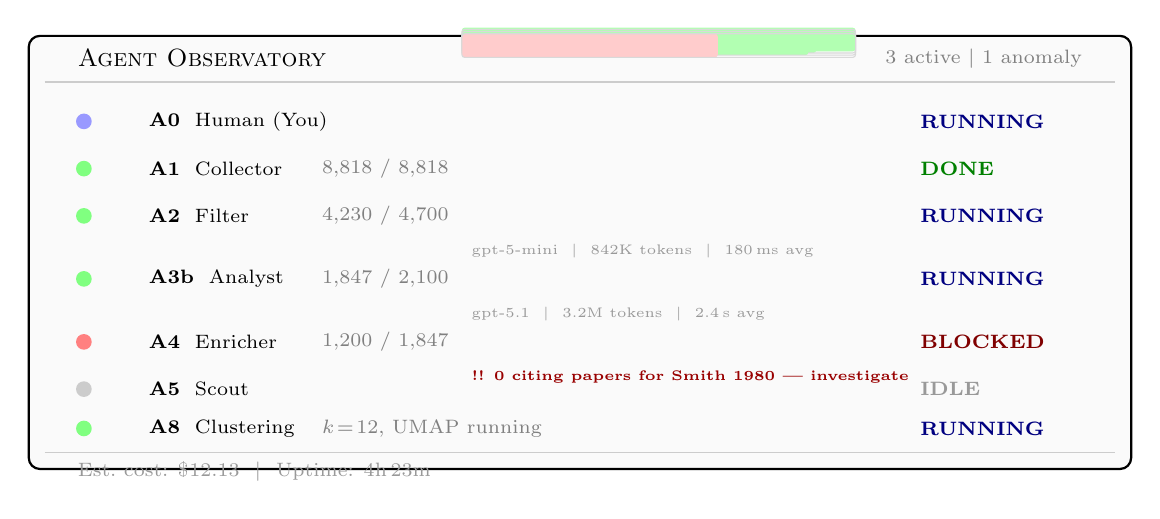
\begin{tikzpicture}

  %% ── Dashboard frame ────────────────────────────────────────
  \node[draw, thick, rounded corners=4pt,
        minimum width=14cm, minimum height=5.5cm,
        fill=black!2, anchor=north] (frame) at (0, 0) {};

  %% ── Header ─────────────────────────────────────────────────
  \node[font=\small\scshape, anchor=west] at (-6.5, -0.3)
    {\textsc{Agent Observatory}};
  \node[font=\scriptsize, text=black!50, anchor=east] at (6.5, -0.3)
    {3 active~\textbar~1 anomaly};

  \draw[thin, black!20] (-6.8, -0.6) -- (6.8, -0.6);

  %% ── Helper: progress bar macro ─────────────────────────────
  %% Usage: \pgfmathsetmacro{\prog}{fraction}
  %% Then draw filled + empty segments

  %% ── Agent rows ─────────────────────────────────────────────
  % Column positions
  \def\xcol{-6.3}     % status icon
  \def\xname{-5.6}    % agent name
  \def\xbar{-1.5}     % progress bar start
  \def\xbarend{3.5}   % progress bar end
  \def\xstatus{4.2}   % status label
  \def\xdetail{-1.5}  % detail line

  % Row 1: A0 Human
  \def\yrow{-1.1}
  \node[fill=blue!40, circle, inner sep=2pt] at (\xcol, \yrow) {};
  \node[font=\scriptsize, anchor=west] at (\xname, \yrow)
    {\textbf{A0}~~Human (You)};
  \node[font=\scriptsize\bfseries, text=blue!50!black,
        anchor=west] at (\xstatus, \yrow) {RUNNING};

  % Row 2: A1 Collector (complete)
  \def\yrow{-1.7}
  \node[fill=green!50, circle, inner sep=2pt] at (\xcol, \yrow) {};
  \node[font=\scriptsize, anchor=west] at (\xname, \yrow)
    {\textbf{A1}~~Collector};
  \node[font=\scriptsize, anchor=west, text=black!50] at (\xname+2.2, \yrow)
    {8{,}818 / 8{,}818};
  % Full bar
  \fill[green!30, rounded corners=1pt]
    (\xbar, \yrow-1.5mm) rectangle (\xbarend, \yrow+1.5mm);
  \node[font=\scriptsize\bfseries, text=green!50!black,
        anchor=west] at (\xstatus, \yrow) {DONE};

  % Row 3: A2 Filter (in progress)
  \def\yrow{-2.3}
  \node[fill=green!50, circle, inner sep=2pt] at (\xcol, \yrow) {};
  \node[font=\scriptsize, anchor=west] at (\xname, \yrow)
    {\textbf{A2}~~Filter};
  \node[font=\scriptsize, anchor=west, text=black!50] at (\xname+2.2, \yrow)
    {4{,}230 / 4{,}700};
  % Partial bar (90%)
  \fill[green!30, rounded corners=1pt]
    (\xbar, \yrow-1.5mm) rectangle (\xbar+0.9*5, \yrow+1.5mm);
  \draw[thin, black!15, rounded corners=1pt]
    (\xbar, \yrow-1.5mm) rectangle (\xbarend, \yrow+1.5mm);
  \node[font=\scriptsize\bfseries, text=blue!50!black,
        anchor=west] at (\xstatus, \yrow) {RUNNING};
  % Detail line
  \node[font=\tiny, text=black!40, anchor=west] at (\xdetail, \yrow-0.45)
    {gpt-5-mini~~\textbar~~842K tokens~~\textbar~~180\,ms avg};

  % Row 4: A3b Analyst (in progress)
  \def\yrow{-3.1}
  \node[fill=green!50, circle, inner sep=2pt] at (\xcol, \yrow) {};
  \node[font=\scriptsize, anchor=west] at (\xname, \yrow)
    {\textbf{A3b}~~Analyst};
  \node[font=\scriptsize, anchor=west, text=black!50] at (\xname+2.2, \yrow)
    {1{,}847 / 2{,}100};
  % Partial bar (88%)
  \fill[green!30, rounded corners=1pt]
    (\xbar, \yrow-1.5mm) rectangle (\xbar+0.88*5, \yrow+1.5mm);
  \draw[thin, black!15, rounded corners=1pt]
    (\xbar, \yrow-1.5mm) rectangle (\xbarend, \yrow+1.5mm);
  \node[font=\scriptsize\bfseries, text=blue!50!black,
        anchor=west] at (\xstatus, \yrow) {RUNNING};
  \node[font=\tiny, text=black!40, anchor=west] at (\xdetail, \yrow-0.45)
    {gpt-5.1~~\textbar~~3.2M tokens~~\textbar~~2.4\,s avg};

  % Row 5: A4 Enricher (BLOCKED — anomaly)
  \def\yrow{-3.9}
  \node[fill=red!50, circle, inner sep=2pt] at (\xcol, \yrow) {};
  \node[font=\scriptsize, anchor=west] at (\xname, \yrow)
    {\textbf{A4}~~Enricher};
  \node[font=\scriptsize, anchor=west, text=black!50] at (\xname+2.2, \yrow)
    {1{,}200 / 1{,}847};
  % Partial bar (65%)
  \fill[red!20, rounded corners=1pt]
    (\xbar, \yrow-1.5mm) rectangle (\xbar+0.65*5, \yrow+1.5mm);
  \draw[thin, black!15, rounded corners=1pt]
    (\xbar, \yrow-1.5mm) rectangle (\xbarend, \yrow+1.5mm);
  \node[font=\scriptsize\bfseries, text=red!50!black,
        anchor=west] at (\xstatus, \yrow) {BLOCKED};
  \node[font=\tiny\bfseries, text=red!60!black, anchor=west]
    at (\xdetail, \yrow-0.45)
    {!! 0 citing papers for Smith 1980 --- investigate};

  % Row 6: A5 Scout (idle)
  \def\yrow{-4.5}
  \node[fill=black!20, circle, inner sep=2pt] at (\xcol, \yrow) {};
  \node[font=\scriptsize, anchor=west] at (\xname, \yrow)
    {\textbf{A5}~~Scout};
  \node[font=\scriptsize\bfseries, text=black!40,
        anchor=west] at (\xstatus, \yrow) {IDLE};

  % Row 7: A8 Clustering (running)
  \def\yrow{-5.0}
  \node[fill=green!50, circle, inner sep=2pt] at (\xcol, \yrow) {};
  \node[font=\scriptsize, anchor=west] at (\xname, \yrow)
    {\textbf{A8}~~Clustering};
  \node[font=\scriptsize, anchor=west, text=black!50] at (\xname+2.2, \yrow)
    {$k\!=\!12$, UMAP running};
  \node[font=\scriptsize\bfseries, text=blue!50!black,
        anchor=west] at (\xstatus, \yrow) {RUNNING};

  %% ── Footer ─────────────────────────────────────────────────
  \draw[thin, black!20] (-6.8, -5.3) -- (6.8, -5.3);
  \node[font=\scriptsize, text=black!40, anchor=west] at (-6.5, -5.55)
    {Est.\ cost: \$12.13~~\textbar~~Uptime: 4h\,23m};

\end{tikzpicture}
\caption{Pattern~5: The Observatory.  Inspired by Nii's blackboard
control shell~\protect\cite{nii1986blackboard}, the Observatory
provides system-level situational awareness: agent status, progress,
model/token costs, and anomaly detection.  Agent~A4's block
(0~citing papers for Smith 1980) is surfaced as an actionable
alert requiring Agent~0 investigation.}
\label{fig:observatory}
\end{figure*}


%% ════════════════════════════════════════════════════════════════
%% Figure 6: The Dual-Loop Theory
%% (Pirolli & Card → Agent 0 architecture)
%% ════════════════════════════════════════════════════════════════

\begin{figure*}[t]
\centering
\begin{tikzpicture}[node distance=5mm]

  %% ── UPPER LOOP: HUMAN (Agent 0) ───────────────────────────
  \node[draw, thick, rounded corners=4pt, fill=blue!5,
        minimum width=5.8cm, minimum height=3.4cm,
        anchor=north west] (upper) at (0, 0) {};

  \node[font=\small\scshape, text=blue!50!black,
        anchor=north west] at (0.3, -0.15)
    {Upper Loop --- Human (Agent 0)};

  \node[font=\scriptsize, anchor=north west, align=left,
        text width=5cm] at (0.3, -0.7)
    {Form hypotheses\\
     Make judgments\\
     Connect concepts\\
     Draw conclusions\\
     Set research direction};

  %% ── LOWER LOOP: AGENTS (A1-A8) ────────────────────────────
  \node[draw, thick, rounded corners=4pt, fill=green!5,
        minimum width=5.8cm, minimum height=3.4cm,
        below=12mm of upper.south west, anchor=north west] (lower) {};

  \node[font=\small\scshape, text=green!50!black,
        anchor=north west] at ([xshift=3mm, yshift=-1.5mm]lower.north west)
    {Lower Loop --- Agents (A1--A8)};

  \node[font=\scriptsize, anchor=north west, align=left,
        text width=5cm]
    at ([xshift=3mm, yshift=-7mm]lower.north west)
    {Search literature (A1)\\
     Filter relevance (A2)\\
     Extract concepts (A3b)\\
     Expand citations (A4)\\
     Find code (A5)\\
     Cluster knowledge (A8)};

  %% ── Bidirectional arrows between loops ─────────────────────
  \draw[hitl/flow, blue!50!black, line width=1.2pt]
    ([xshift=15mm]upper.south) --
    node[left, font=\scriptsize, text=blue!50!black, align=right]
      {redirects\\agents}
    ([xshift=15mm]lower.north);

  \draw[hitl/flow, green!50!black, line width=1.2pt]
    ([xshift=40mm]lower.north) --
    node[right, font=\scriptsize, text=green!50!black, align=left]
      {feeds\\discoveries}
    ([xshift=40mm]upper.south);

  %% ── INTERFACE COLUMN (right) ───────────────────────────────
  \node[draw, thick, rounded corners=4pt, fill=black!3,
        minimum width=4cm, minimum height=7.8cm,
        anchor=north west] (iface)
    at ([xshift=18mm]upper.north east) {};

  \node[font=\small\scshape, text=black!50,
        anchor=north] at ([yshift=-2mm]iface.north)
    {Interface Patterns};

  % Upper-loop patterns
  \node[draw, thin, rounded corners=2pt, fill=blue!6,
        font=\scriptsize, inner sep=3pt, text width=3cm,
        align=left, anchor=north west] (ip1)
    at ([xshift=3mm, yshift=-10mm]iface.north west)
    {Canvas (P1)\\Checkpoints (P2)\\Reasoning Tree (P4)};

  % Lower-loop patterns
  \node[draw, thin, rounded corners=2pt, fill=green!6,
        font=\scriptsize, inner sep=3pt, text width=3cm,
        align=left, below=8mm of ip1] (ip2)
    {Foraging Feed (P6)\\Observatory (P5)\\Provenance Flow (P3)};

  %% ── Interface ↔ Loop connections ───────────────────────────
  \draw[hitl/thinflow, blue!40, dashed]
    (ip1.west) -- ++(-8mm, 0) |- ([yshift=-10mm]upper.east);
  \draw[hitl/thinflow, green!40, dashed]
    (ip2.west) -- ++(-8mm, 0) |- ([yshift=10mm]lower.east);

  % Labels on connections
  \node[font=\tiny, text=blue!40, anchor=south, rotate=0]
    at ([xshift=-2mm, yshift=-10mm]upper.east) {human tools};
  \node[font=\tiny, text=green!40, anchor=north, rotate=0]
    at ([xshift=-2mm, yshift=10mm]lower.east) {agent views};

  %% ── Co-temporal annotation ─────────────────────────────────
  \node[draw, thin, rounded corners=3pt, fill=yellow!8,
        font=\scriptsize\itshape, inner sep=4pt,
        text width=3.4cm, align=center,
        below=6mm of ip2] (note)
    {Both loops run \textbf{co-temporally}.\\
     Agents forage while human\\
     makes sense. Human redirects\\
     based on emerging understanding.};

\end{tikzpicture}
\caption{The Dual-Loop Architecture (after Pirolli \&
Card~\protect\cite{pirolli2005sensemaking}).  The upper loop
(human sensemaking) and lower loop (agent foraging) run
co-temporally, connected through six interface patterns.  The
human directs agents based on emerging understanding; agents
feed discoveries that reshape the human's conceptual landscape.
This is the core operational model for cointelligence.}
\label{fig:dual-loop}
\end{figure*}
  (from main.tex)
%%
%% Required packages — add to main.tex preamble:
%%
%%   \usepackage{tikz}
%%   \usetikzlibrary{positioning, arrows.meta, shapes.geometric,
%%                    fit, backgrounds, decorations.pathreplacing,
%%                    calc, patterns}
%%
%% Each figure can be used independently — copy the relevant
%% \begin{figure*}...\end{figure*} block into main.tex as needed.
%% ────────────────────────────────────────────────────────────────


%% ════════════════════════════════════════════════════════════════
%% Shared style definitions
%% ════════════════════════════════════════════════════════════════

\tikzset{
  % Panel frames
  hitl/panel/.style={
    draw, thick, rounded corners=3pt, inner sep=5pt},
  % Feed items (scrolling list entries)
  hitl/feeditem/.style={
    draw, thin, rounded corners=2pt, fill=black!4,
    text width=2.5cm, font=\scriptsize, inner sep=3pt, align=left},
  % Canvas nodes (spatial sensemaking)
  hitl/cnode/.style={
    draw, rounded corners=3pt, font=\scriptsize,
    inner sep=4pt, align=center},
  % Phase boxes (cognitive forcing flow)
  hitl/phase/.style={
    draw, thick, rounded corners=4pt,
    minimum width=3.4cm, inner sep=5pt, align=left},
  % Agent circles (provenance DAG)
  hitl/agent/.style={
    draw, thick, circle, minimum size=9mm,
    font=\footnotesize\bfseries, inner sep=0pt},
  % Tree nodes (reasoning tree)
  hitl/tnode/.style={
    draw, thin, rounded corners=2pt, fill=black!4,
    font=\scriptsize, inner sep=3pt, anchor=west},
  % Status markers
  hitl/ok/.style={fill=green!15, draw=green!50!black},
  hitl/warn/.style={fill=yellow!15, draw=yellow!50!black},
  hitl/err/.style={fill=red!15, draw=red!50!black},
  % Arrows
  hitl/flow/.style={
    -{Stealth[length=5pt, width=4pt]}, thick},
  hitl/thinflow/.style={
    -{Stealth[length=4pt, width=3pt]}, thin},
  hitl/biflow/.style={
    {Stealth[length=4pt]}-{Stealth[length=4pt]}, thick},
  % Labels
  hitl/sec/.style={font=\footnotesize\scshape, text=black!60},
  hitl/sub/.style={font=\scriptsize, text=black!50},
}


%% ════════════════════════════════════════════════════════════════
%% Figure 1: Pattern 1+6 — Sensemaking Workspace
%% (Multilevel Canvas + Dual Sensemaking Loop)
%% ════════════════════════════════════════════════════════════════

\begin{figure*}[t]
\centering
\begin{tikzpicture}[node distance=3pt]

  %% ── FORAGING FEED (left panel) ──────────────────────────────
  \node[hitl/sec] (ftitle) at (0, 5) {\textsc{Foraging Feed}};
  \node[hitl/sub, below=0pt of ftitle] (fsub) {(Agent Lower Loop)};

  \node[hitl/feeditem] (f1) at (0, 3.5)
    {\textbullet~\textbf{A3b}~~2\,min ago\\
     LbMAS: ``shared workspace''\\
     13--57\% improvement};
  \node[hitl/feeditem, below=3pt of f1] (f2)
    {\textbullet~\textbf{A4}~~3\,min ago\\
     Nii 1986: 2{,}341 cites\\
     modernity\,$=0.02$};
  \node[hitl/feeditem, below=3pt of f2] (f3)
    {\textbullet~\textbf{A8}~~5\,min ago\\
     Cluster 7 relabeled\\
     ``Shared State Coord''};
  \node[hitl/feeditem, below=3pt of f3] (f4)
    {\textbullet~\textbf{A3b}~~8\,min ago\\
     freephdlabor: workspace\\
     $=$ blackboard};

  % Feed frame
  \begin{scope}[on background layer]
    \node[hitl/panel, fill=black!2,
          fit=(ftitle)(f4), inner sep=8pt] (fbox) {};
  \end{scope}

  %% ── SENSEMAKING CANVAS (right panel) ───────────────────────
  \node[hitl/sec] (ctitle) at (7.2, 5) {\textsc{Sensemaking Canvas}};
  \node[hitl/sub, below=0pt of ctitle] (csub) {(Human Upper Loop)};

  % Thesis node (highest abstraction)
  \node[hitl/cnode, fill=blue!10, minimum width=2.6cm,
        text width=2.4cm, align=center] (thesis) at (6, 3.5)
    {\textbf{THESIS}\\Modern MAS fail from\\missing coordination};

  % Cluster node (mid abstraction)
  \node[hitl/cnode, fill=green!8, minimum width=2.2cm,
        text width=2cm, align=center] (cluster) at (6.5, 1.8)
    {\textbf{CLUSTER}\\Lost Canary:\\Blackboard arch.};

  % Paper nodes (leaf level)
  \node[hitl/cnode, fill=yellow!8, text width=1.6cm,
        align=center] (p1) at (5.2, 0.3)
    {\textbf{PAPER}\\LbMAS:\\shared workspace};
  \node[hitl/cnode, fill=yellow!8, text width=1.6cm,
        align=center] (p2) at (8.2, 0.5)
    {\textbf{PAPER}\\freephdlabor:\\workspace};

  % Conceptual links (proximity = relatedness)
  \draw[hitl/thinflow, black!30] (thesis) -- (cluster);
  \draw[hitl/thinflow, black!30] (cluster) -- (p1);
  \draw[hitl/thinflow, black!30] (cluster) -- (p2);

  % Spatial annotation
  \node[hitl/sub, rotate=90] at (9.4, 2)
    {spatial proximity $=$ conceptual link};

  % Canvas frame
  \begin{scope}[on background layer]
    \node[hitl/panel, fill=blue!2,
          fit=(ctitle)(p1)(p2)(thesis),
          inner xsep=12pt, inner ysep=8pt,
          minimum width=7cm, minimum height=5.5cm] (cbox) {};
  \end{scope}

  %% ── FEED → CANVAS arrow ────────────────────────────────────
  \draw[hitl/flow, blue!50!black]
    ([yshift=5mm]fbox.east) --
    node[above, font=\scriptsize, text=blue!50!black] {promote}
    ([yshift=5mm]cbox.west);

  %% ── ZOOM LEVELS (bottom strip) ─────────────────────────────
  \node[draw, rounded corners=3pt, fill=blue!8,
        minimum width=2.2cm, minimum height=8mm,
        font=\scriptsize, align=center] (z1) at (2.2, -1.6)
    {\textbf{Thesis} (forest)};
  \node[draw, rounded corners=3pt, fill=green!8,
        minimum width=2.2cm, minimum height=8mm,
        font=\scriptsize, align=center,
        right=6mm of z1] (z2)
    {\textbf{Cluster} (tree)};
  \node[draw, rounded corners=3pt, fill=yellow!8,
        minimum width=2.2cm, minimum height=8mm,
        font=\scriptsize, align=center,
        right=6mm of z2] (z3)
    {\textbf{Paper} (leaf)};

  \draw[hitl/biflow, black!40] (z1) -- (z2);
  \draw[hitl/biflow, black!40] (z2) -- (z3);
  \node[hitl/sub, below=2pt of z1] {zoomed out};
  \node[hitl/sub, below=2pt of z3] {zoomed in};

  % Brace for zoom label
  \draw[decorate, decoration={brace, amplitude=4pt, mirror},
        black!40]
    ([yshift=-12mm]z1.south west) -- ([yshift=-12mm]z3.south east)
    node[midway, below=5pt, font=\scriptsize, text=black!50]
    {semantic zoom (Sensecape)};

\end{tikzpicture}
\caption{Pattern~1+6: The Sensemaking Workspace.  The foraging feed
(left) streams agent discoveries from the lower loop; the human
promotes items to a spatial canvas (right) where proximity encodes
conceptual relatedness.  Three semantic zoom levels (bottom) allow
navigation from thesis-level abstractions down to individual paper
evidence, following Suh et~al.'s Sensecape~\protect\cite{suh2023sensecape}
and Pirolli \& Card's dual-loop sensemaking model~\protect\cite{pirolli2005sensemaking}.}
\label{fig:sensemaking}
\end{figure*}


%% ════════════════════════════════════════════════════════════════
%% Figure 2: Pattern 2 — Cognitive Forcing Functions
%% (Judgment Checkpoint: commit-before-reveal protocol)
%% ════════════════════════════════════════════════════════════════

\begin{figure*}[t]
\centering
\begin{tikzpicture}[node distance=6mm]

  %% ── Phase 1: EVIDENCE ──────────────────────────────────────
  \node[hitl/phase, fill=black!3, minimum height=3.2cm] (ph1) at (0, 0)
    {\footnotesize\textsc{Phase 1: Evidence}\\[3pt]
     \scriptsize
     \begin{tabular}{@{}l@{}}
       Evidence presented:\\[1pt]
       \textbullet~Nii 1986: 2{,}341 cites\\
       \textbullet~LbMAS: no citation\\
       \textbullet~Cluster 7: 12 papers\\[4pt]
       AI assessment:\\[-1pt]
     \end{tabular}};

  % Hidden AI overlay (hatched box)
  \node[draw, thick, fill=black!8,
        pattern=north east lines, pattern color=black!20,
        minimum width=2.4cm, minimum height=6mm,
        rounded corners=2pt,
        font=\scriptsize\itshape, text=black!50]
    (hidden) at ([yshift=-12mm]ph1.center)
    {~HIDDEN~};

  %% ── Phase 2: COMMIT ───────────────────────────────────────
  \node[hitl/phase, fill=blue!5, minimum height=3.2cm,
        right=8mm of ph1] (ph2)
    {\footnotesize\textsc{Phase 2: Commit}\\[3pt]
     \scriptsize
     \begin{tabular}{@{}l@{}}
       Human writes own\\
       assessment \emph{first}:\\[2pt]
       \fbox{\parbox{2.2cm}{\scriptsize
         ``I think the blackboard\\
         is genuinely lost\\
         because\ldots''}}\\[3pt]
       Confidence: 80\%\\[2pt]
       {[\,\textsc{commit judgment}\,]}
     \end{tabular}};

  %% ── Phase 3+4: REVEAL + DELIBERATE ────────────────────────
  \node[hitl/phase, fill=green!5, minimum height=3.2cm,
        right=8mm of ph2] (ph34)
    {\footnotesize\textsc{Phase 3+4: Reveal \& Deliberate}\\[3pt]
     \scriptsize
     \begin{tabular}{@{}l@{}}
       \textbf{Human}: ``genuinely lost\ldots''\\
       Confidence: 80\%\\[2pt]
       \textbf{AI}: ``GENUINELY LOST.\\
       ~~~~Modernity 0.02\ldots''\\
       Confidence: 92\%\\[3pt]
       {[\,Agree\,]~~[\,Partial\,]~~[\,Override\,]}
     \end{tabular}};

  %% ── Phase arrows ───────────────────────────────────────────
  \draw[hitl/flow] (ph1) -- (ph2);
  \draw[hitl/flow] (ph2) -- node[above, font=\scriptsize,
    text=black!50] {commit} (ph34);

  %% ── Key insight callout ────────────────────────────────────
  \draw[decorate, decoration={brace, amplitude=5pt, mirror},
        thick, blue!50!black]
    ([yshift=-3mm]ph1.south west) -- ([yshift=-3mm]ph2.south east)
    node[midway, below=7pt, font=\scriptsize,
         text=blue!50!black, align=center]
    {Human commits \emph{before}\\seeing AI (the forcing function)};

  %% ── Comparison: Standard XAI vs. CFF (bottom) ─────────────
  \node[draw, rounded corners=3pt, fill=red!5,
        minimum width=4.5cm, minimum height=1.2cm,
        font=\scriptsize, align=center] (sys1) at (1.8, -3.5)
    {\textbf{Standard XAI} (System~1)\\[1pt]
     AI says X $\to$ Human accepts\\
     (overreliance, fast heuristic)};
  \node[draw, rounded corners=3pt, fill=green!5,
        minimum width=4.5cm, minimum height=1.2cm,
        font=\scriptsize, align=center,
        right=8mm of sys1] (sys2)
    {\textbf{Cognitive Forcing} (System~2)\\[1pt]
     Evidence $\to$ Human commits $\to$ AI revealed\\
     (analytical engagement)};

  \node[font=\scriptsize\bfseries, text=black!40] at
    ($(sys1.east)!0.5!(sys2.west)$) {vs.};

\end{tikzpicture}
\caption{Pattern~2: Cognitive Forcing Functions.  The human must
commit their own judgment (Phase~2) \emph{before} seeing the AI
assessment (Phase~3), activating System~2 analytical reasoning
instead of System~1 anchoring.  This reduces overreliance
($p<.001$, $N\!=\!199$)~\protect\cite{bucinca2021trust}.  Bottom:
the forcing function replaces the standard XAI accept-or-reject
with a commit-then-compare protocol.}
\label{fig:cff}
\end{figure*}


%% ════════════════════════════════════════════════════════════════
%% Figure 3: Pattern 3 — Provenance Flow
%% (Agent pipeline DAG with edge annotations)
%% ════════════════════════════════════════════════════════════════

\begin{figure*}[t]
\centering
\begin{tikzpicture}[node distance=14mm]

  %% ── Agent nodes ────────────────────────────────────────────
  \node[hitl/agent, fill=blue!10] (a0)
    {A0};
  \node[hitl/agent, fill=green!10, right=of a0] (a1)
    {A1};
  \node[hitl/agent, fill=green!10, right=of a1] (a2)
    {A2};
  \node[hitl/agent, fill=green!10, right=18mm of a2] (a3b)
    {A3b};
  \node[hitl/agent, fill=green!10, above right=6mm and 14mm of a3b] (a4)
    {A4};
  \node[hitl/agent, fill=green!10, below right=6mm and 14mm of a3b] (a8)
    {A8};
  \node[hitl/agent, fill=blue!10, right=30mm of a3b] (a0end)
    {A0};

  %% ── Agent labels ───────────────────────────────────────────
  \node[hitl/sub, below=3pt of a0]  {Human};
  \node[hitl/sub, below=3pt of a1]  {Collector};
  \node[hitl/sub, below=3pt of a2]  {Filter};
  \node[hitl/sub, below=3pt of a3b] {Analyst};
  \node[hitl/sub, above=3pt of a4]  {Enricher};
  \node[hitl/sub, below=3pt of a8]  {Cluster};
  \node[hitl/sub, below=3pt of a0end] {Finding};

  %% ── Edges with annotations ─────────────────────────────────
  \draw[hitl/flow] (a0) --
    node[above, font=\scriptsize] {seed paper}
    (a1);
  \draw[hitl/flow] (a1) --
    node[above, font=\scriptsize] {200 papers}
    (a2);
  \draw[hitl/flow] (a2) --
    node[above, font=\scriptsize] {47 relevant}
    (a3b);
  \draw[hitl/flow] (a3b) --
    node[above, font=\scriptsize, sloped] {enrichment}
    (a4);
  \draw[hitl/flow] (a3b) --
    node[below, font=\scriptsize, sloped] {$k\!=\!12$}
    (a8);
  \draw[hitl/flow] (a4) --
    node[above, font=\scriptsize, sloped] {mod\,$=0.02$}
    (a0end);
  \draw[hitl/flow] (a8) --
    node[below, font=\scriptsize, sloped] {cluster \#7}
    (a0end);

  %% ── A3b detail box ─────────────────────────────────────────
  \node[draw, thin, rounded corners=3pt, fill=black!3,
        font=\scriptsize, align=left,
        below=12mm of a3b, text width=4cm] (detail)
    {47 papers $\to$ 12 ``shared workspace''\\
     0 cite Nii. Lost Canary: \textbf{STRONG}\\
     Tokens: 180K~~Confidence: 92\%};
  \draw[hitl/thinflow, black!30] (a3b) -- (detail);

  %% ── Finding box ────────────────────────────────────────────
  \node[draw, thick, rounded corners=3pt, fill=blue!8,
        font=\scriptsize, align=center,
        below=8mm of a0end, text width=4cm] (finding)
    {\textbf{FINDING}: Blackboard is a Lost Canary.\\
     2{,}341 citations. Modernity\,$=0.02$.};
  \draw[hitl/thinflow, blue!50!black] (a0end) -- (finding);

  %% ── Provenance highlight annotation ────────────────────────
  \node[font=\scriptsize\itshape, text=black!40,
        below=6mm of detail]
    {Click any node $\to$ highlights provenance path back to origin};

\end{tikzpicture}
\caption{Pattern~3: Provenance Flow.  Every finding in the pipeline
carries a full audit trail through the agent DAG.  Agent~0 (human)
provides the seed; Agents~1--8 process in stages with annotated
handoffs showing paper counts, token costs, and confidence.  Click
any node to trace the evidence chain back to its origin, inspired
by ChainForge~\protect\cite{arawjo2024chainforge}.}
\label{fig:provenance}
\end{figure*}


%% ════════════════════════════════════════════════════════════════
%% Figure 4: Pattern 4 — Reasoning Tree Manipulation
%% (Editable agent reasoning with node-level controls)
%% ════════════════════════════════════════════════════════════════

\begin{figure*}[t]
\centering
\begin{tikzpicture}[
  level distance=11mm,
  sibling distance=8mm,
  every node/.style={font=\scriptsize},
  edge from parent/.style={draw, thin, black!50},
]

  %% ── Tree root ──────────────────────────────────────────────
  \node[hitl/tnode, hitl/ok, text width=7cm]
    (root) {Query: ``Is blackboard architecture cited by LbMAS?''
            \hfill[\,\textcolor{green!50!black}{ok}\,]};

  %% ── Step 1 ─────────────────────────────────────────────────
  \node[hitl/tnode, hitl/ok, text width=5.5cm,
        below=7mm of root.south west, anchor=north west,
        xshift=8mm] (s1)
    {Step 1: Paper retrieval ---
     ``Retrieved LbMAS (2025). 23 pages.''
     \hfill[\,\textcolor{green!50!black}{ok}\,]};
  \draw[thin, black!50] (root.south west) ++(4mm,0) |- (s1.west);

  %% ── Step 2 ─────────────────────────────────────────────────
  \node[hitl/tnode, hitl/ok, text width=5.5cm,
        below=5mm of s1] (s2)
    {Step 2: Reference extraction
     \hfill[\,\textcolor{green!50!black}{ok}\,]};
  \draw[thin, black!50] (root.south west) ++(4mm,0) |- (s2.west);

  %% ── Step 2 children ────────────────────────────────────────
  \node[hitl/tnode, hitl/ok, text width=4.5cm,
        below=5mm of s2.south west, anchor=north west,
        xshift=8mm] (s2a)
    {Keyword match: 0 for Nii/Erman
     \hfill[\,\textcolor{green!50!black}{ok}\,]};
  \draw[thin, black!50] (s2.south west) ++(4mm,0) |- (s2a.west);

  \node[hitl/tnode, hitl/warn, text width=4.5cm,
        below=5mm of s2a] (s2b)
    {Semantic match: 14 ``shared workspace''
     \hfill[\,\textcolor{yellow!50!black}{warn}\,]};
  \draw[thin, black!50] (s2.south west) ++(4mm,0) |- (s2b.west);

  %% ── Interactive controls on warning node ───────────────────
  \node[draw, thin, rounded corners=2pt, fill=blue!8,
        font=\scriptsize, inner sep=2pt,
        right=5mm of s2b] (ctrl)
    {[\,edit\,]~~[\,regen\,]~~[\,branch\,]};
  \draw[hitl/thinflow, blue!40] (s2b.east) -- (ctrl.west);

  %% ── Step 3 ─────────────────────────────────────────────────
  \node[hitl/tnode, hitl/warn, text width=5.5cm,
        below=5mm of s2b, xshift=-8mm] (s3)
    {Step 3: Concept overlap
     \hfill[\,\textcolor{yellow!50!black}{warn}\,]};
  \draw[thin, black!50] (root.south west) ++(4mm,0) |- (s3.west);

  %% ── Step 3 children ────────────────────────────────────────
  \node[hitl/tnode, hitl/warn, text width=4.2cm,
        below=5mm of s3.south west, anchor=north west,
        xshift=8mm] (s3a)
    {BB data\,$=$\,MATCH, shell\,$=$\,MISS
     \hfill[\,\textcolor{yellow!50!black}{warn}\,]};
  \draw[thin, black!50] (s3.south west) ++(4mm,0) |- (s3a.west);

  \node[hitl/tnode, hitl/err, text width=4.2cm,
        below=5mm of s3a] (s3b)
    {\textbf{REINVENTION WITHOUT ATTRIBUTION}
     \hfill[\,\textcolor{red!50!black}{error}\,]};
  \draw[thin, black!50] (s3.south west) ++(4mm,0) |- (s3b.west);

  %% ── Step 4 ─────────────────────────────────────────────────
  \node[hitl/tnode, hitl/ok, text width=5.5cm,
        below=5mm of s3b, xshift=-8mm] (s4)
    {Step 4: Lost Canary signal \textbf{STRONG}
     \hfill[\,\textcolor{green!50!black}{ok}\,]};
  \draw[thin, black!50] (root.south west) ++(4mm,0) |- (s4.west);

  %% ── Legend ─────────────────────────────────────────────────
  \node[font=\scriptsize, text=black!50, anchor=west]
    at ([xshift=-8mm, yshift=-8mm]s4.south west)
    {Status:
     \textcolor{green!50!black}{\rule{5pt}{5pt}}~ok\quad
     \textcolor{yellow!50!black}{\rule{5pt}{5pt}}~warning\quad
     \textcolor{red!50!black}{\rule{5pt}{5pt}}~error\quad
     \textcolor{blue!50!black}{\rule{5pt}{5pt}}~edited by human};

\end{tikzpicture}
\caption{Pattern~4: Reasoning Tree Manipulation.  Agent~3b's
reasoning chain is exposed as an editable tree, following
Hippo~\protect\cite{pang2025hippo}.  Each node carries a status
marker; warning and error nodes offer interactive controls
(\emph{edit}, \emph{regen}, \emph{branch}) enabling the human to
intervene at the specific reasoning step that needs correction,
rather than accepting or rejecting the entire chain.}
\label{fig:reasoning-tree}
\end{figure*}


%% ════════════════════════════════════════════════════════════════
%% Figure 5: Pattern 5 — The Observatory (Control Shell)
%% (System-state dashboard with progress and anomaly detection)
%% ════════════════════════════════════════════════════════════════

\begin{figure*}[t]
\centering
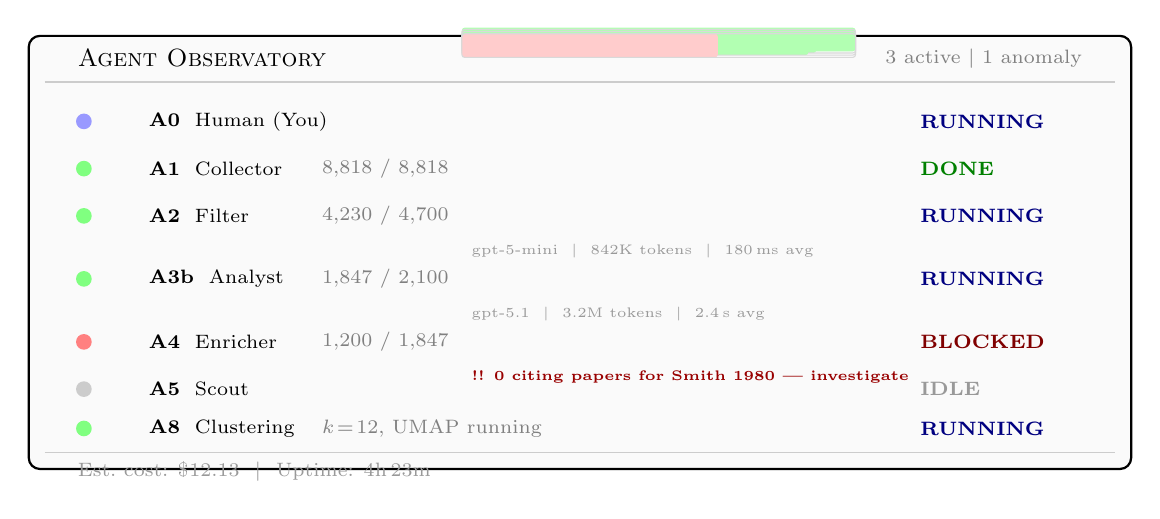
\begin{tikzpicture}

  %% ── Dashboard frame ────────────────────────────────────────
  \node[draw, thick, rounded corners=4pt,
        minimum width=14cm, minimum height=5.5cm,
        fill=black!2, anchor=north] (frame) at (0, 0) {};

  %% ── Header ─────────────────────────────────────────────────
  \node[font=\small\scshape, anchor=west] at (-6.5, -0.3)
    {\textsc{Agent Observatory}};
  \node[font=\scriptsize, text=black!50, anchor=east] at (6.5, -0.3)
    {3 active~\textbar~1 anomaly};

  \draw[thin, black!20] (-6.8, -0.6) -- (6.8, -0.6);

  %% ── Helper: progress bar macro ─────────────────────────────
  %% Usage: \pgfmathsetmacro{\prog}{fraction}
  %% Then draw filled + empty segments

  %% ── Agent rows ─────────────────────────────────────────────
  % Column positions
  \def\xcol{-6.3}     % status icon
  \def\xname{-5.6}    % agent name
  \def\xbar{-1.5}     % progress bar start
  \def\xbarend{3.5}   % progress bar end
  \def\xstatus{4.2}   % status label
  \def\xdetail{-1.5}  % detail line

  % Row 1: A0 Human
  \def\yrow{-1.1}
  \node[fill=blue!40, circle, inner sep=2pt] at (\xcol, \yrow) {};
  \node[font=\scriptsize, anchor=west] at (\xname, \yrow)
    {\textbf{A0}~~Human (You)};
  \node[font=\scriptsize\bfseries, text=blue!50!black,
        anchor=west] at (\xstatus, \yrow) {RUNNING};

  % Row 2: A1 Collector (complete)
  \def\yrow{-1.7}
  \node[fill=green!50, circle, inner sep=2pt] at (\xcol, \yrow) {};
  \node[font=\scriptsize, anchor=west] at (\xname, \yrow)
    {\textbf{A1}~~Collector};
  \node[font=\scriptsize, anchor=west, text=black!50] at (\xname+2.2, \yrow)
    {8{,}818 / 8{,}818};
  % Full bar
  \fill[green!30, rounded corners=1pt]
    (\xbar, \yrow-1.5mm) rectangle (\xbarend, \yrow+1.5mm);
  \node[font=\scriptsize\bfseries, text=green!50!black,
        anchor=west] at (\xstatus, \yrow) {DONE};

  % Row 3: A2 Filter (in progress)
  \def\yrow{-2.3}
  \node[fill=green!50, circle, inner sep=2pt] at (\xcol, \yrow) {};
  \node[font=\scriptsize, anchor=west] at (\xname, \yrow)
    {\textbf{A2}~~Filter};
  \node[font=\scriptsize, anchor=west, text=black!50] at (\xname+2.2, \yrow)
    {4{,}230 / 4{,}700};
  % Partial bar (90%)
  \fill[green!30, rounded corners=1pt]
    (\xbar, \yrow-1.5mm) rectangle (\xbar+0.9*5, \yrow+1.5mm);
  \draw[thin, black!15, rounded corners=1pt]
    (\xbar, \yrow-1.5mm) rectangle (\xbarend, \yrow+1.5mm);
  \node[font=\scriptsize\bfseries, text=blue!50!black,
        anchor=west] at (\xstatus, \yrow) {RUNNING};
  % Detail line
  \node[font=\tiny, text=black!40, anchor=west] at (\xdetail, \yrow-0.45)
    {gpt-5-mini~~\textbar~~842K tokens~~\textbar~~180\,ms avg};

  % Row 4: A3b Analyst (in progress)
  \def\yrow{-3.1}
  \node[fill=green!50, circle, inner sep=2pt] at (\xcol, \yrow) {};
  \node[font=\scriptsize, anchor=west] at (\xname, \yrow)
    {\textbf{A3b}~~Analyst};
  \node[font=\scriptsize, anchor=west, text=black!50] at (\xname+2.2, \yrow)
    {1{,}847 / 2{,}100};
  % Partial bar (88%)
  \fill[green!30, rounded corners=1pt]
    (\xbar, \yrow-1.5mm) rectangle (\xbar+0.88*5, \yrow+1.5mm);
  \draw[thin, black!15, rounded corners=1pt]
    (\xbar, \yrow-1.5mm) rectangle (\xbarend, \yrow+1.5mm);
  \node[font=\scriptsize\bfseries, text=blue!50!black,
        anchor=west] at (\xstatus, \yrow) {RUNNING};
  \node[font=\tiny, text=black!40, anchor=west] at (\xdetail, \yrow-0.45)
    {gpt-5.1~~\textbar~~3.2M tokens~~\textbar~~2.4\,s avg};

  % Row 5: A4 Enricher (BLOCKED — anomaly)
  \def\yrow{-3.9}
  \node[fill=red!50, circle, inner sep=2pt] at (\xcol, \yrow) {};
  \node[font=\scriptsize, anchor=west] at (\xname, \yrow)
    {\textbf{A4}~~Enricher};
  \node[font=\scriptsize, anchor=west, text=black!50] at (\xname+2.2, \yrow)
    {1{,}200 / 1{,}847};
  % Partial bar (65%)
  \fill[red!20, rounded corners=1pt]
    (\xbar, \yrow-1.5mm) rectangle (\xbar+0.65*5, \yrow+1.5mm);
  \draw[thin, black!15, rounded corners=1pt]
    (\xbar, \yrow-1.5mm) rectangle (\xbarend, \yrow+1.5mm);
  \node[font=\scriptsize\bfseries, text=red!50!black,
        anchor=west] at (\xstatus, \yrow) {BLOCKED};
  \node[font=\tiny\bfseries, text=red!60!black, anchor=west]
    at (\xdetail, \yrow-0.45)
    {!! 0 citing papers for Smith 1980 --- investigate};

  % Row 6: A5 Scout (idle)
  \def\yrow{-4.5}
  \node[fill=black!20, circle, inner sep=2pt] at (\xcol, \yrow) {};
  \node[font=\scriptsize, anchor=west] at (\xname, \yrow)
    {\textbf{A5}~~Scout};
  \node[font=\scriptsize\bfseries, text=black!40,
        anchor=west] at (\xstatus, \yrow) {IDLE};

  % Row 7: A8 Clustering (running)
  \def\yrow{-5.0}
  \node[fill=green!50, circle, inner sep=2pt] at (\xcol, \yrow) {};
  \node[font=\scriptsize, anchor=west] at (\xname, \yrow)
    {\textbf{A8}~~Clustering};
  \node[font=\scriptsize, anchor=west, text=black!50] at (\xname+2.2, \yrow)
    {$k\!=\!12$, UMAP running};
  \node[font=\scriptsize\bfseries, text=blue!50!black,
        anchor=west] at (\xstatus, \yrow) {RUNNING};

  %% ── Footer ─────────────────────────────────────────────────
  \draw[thin, black!20] (-6.8, -5.3) -- (6.8, -5.3);
  \node[font=\scriptsize, text=black!40, anchor=west] at (-6.5, -5.55)
    {Est.\ cost: \$12.13~~\textbar~~Uptime: 4h\,23m};

\end{tikzpicture}
\caption{Pattern~5: The Observatory.  Inspired by Nii's blackboard
control shell~\protect\cite{nii1986blackboard}, the Observatory
provides system-level situational awareness: agent status, progress,
model/token costs, and anomaly detection.  Agent~A4's block
(0~citing papers for Smith 1980) is surfaced as an actionable
alert requiring Agent~0 investigation.}
\label{fig:observatory}
\end{figure*}


%% ════════════════════════════════════════════════════════════════
%% Figure 6: The Dual-Loop Theory
%% (Pirolli & Card → Agent 0 architecture)
%% ════════════════════════════════════════════════════════════════

\begin{figure*}[t]
\centering
\begin{tikzpicture}[node distance=5mm]

  %% ── UPPER LOOP: HUMAN (Agent 0) ───────────────────────────
  \node[draw, thick, rounded corners=4pt, fill=blue!5,
        minimum width=5.8cm, minimum height=3.4cm,
        anchor=north west] (upper) at (0, 0) {};

  \node[font=\small\scshape, text=blue!50!black,
        anchor=north west] at (0.3, -0.15)
    {Upper Loop --- Human (Agent 0)};

  \node[font=\scriptsize, anchor=north west, align=left,
        text width=5cm] at (0.3, -0.7)
    {Form hypotheses\\
     Make judgments\\
     Connect concepts\\
     Draw conclusions\\
     Set research direction};

  %% ── LOWER LOOP: AGENTS (A1-A8) ────────────────────────────
  \node[draw, thick, rounded corners=4pt, fill=green!5,
        minimum width=5.8cm, minimum height=3.4cm,
        below=12mm of upper.south west, anchor=north west] (lower) {};

  \node[font=\small\scshape, text=green!50!black,
        anchor=north west] at ([xshift=3mm, yshift=-1.5mm]lower.north west)
    {Lower Loop --- Agents (A1--A8)};

  \node[font=\scriptsize, anchor=north west, align=left,
        text width=5cm]
    at ([xshift=3mm, yshift=-7mm]lower.north west)
    {Search literature (A1)\\
     Filter relevance (A2)\\
     Extract concepts (A3b)\\
     Expand citations (A4)\\
     Find code (A5)\\
     Cluster knowledge (A8)};

  %% ── Bidirectional arrows between loops ─────────────────────
  \draw[hitl/flow, blue!50!black, line width=1.2pt]
    ([xshift=15mm]upper.south) --
    node[left, font=\scriptsize, text=blue!50!black, align=right]
      {redirects\\agents}
    ([xshift=15mm]lower.north);

  \draw[hitl/flow, green!50!black, line width=1.2pt]
    ([xshift=40mm]lower.north) --
    node[right, font=\scriptsize, text=green!50!black, align=left]
      {feeds\\discoveries}
    ([xshift=40mm]upper.south);

  %% ── INTERFACE COLUMN (right) ───────────────────────────────
  \node[draw, thick, rounded corners=4pt, fill=black!3,
        minimum width=4cm, minimum height=7.8cm,
        anchor=north west] (iface)
    at ([xshift=18mm]upper.north east) {};

  \node[font=\small\scshape, text=black!50,
        anchor=north] at ([yshift=-2mm]iface.north)
    {Interface Patterns};

  % Upper-loop patterns
  \node[draw, thin, rounded corners=2pt, fill=blue!6,
        font=\scriptsize, inner sep=3pt, text width=3cm,
        align=left, anchor=north west] (ip1)
    at ([xshift=3mm, yshift=-10mm]iface.north west)
    {Canvas (P1)\\Checkpoints (P2)\\Reasoning Tree (P4)};

  % Lower-loop patterns
  \node[draw, thin, rounded corners=2pt, fill=green!6,
        font=\scriptsize, inner sep=3pt, text width=3cm,
        align=left, below=8mm of ip1] (ip2)
    {Foraging Feed (P6)\\Observatory (P5)\\Provenance Flow (P3)};

  %% ── Interface ↔ Loop connections ───────────────────────────
  \draw[hitl/thinflow, blue!40, dashed]
    (ip1.west) -- ++(-8mm, 0) |- ([yshift=-10mm]upper.east);
  \draw[hitl/thinflow, green!40, dashed]
    (ip2.west) -- ++(-8mm, 0) |- ([yshift=10mm]lower.east);

  % Labels on connections
  \node[font=\tiny, text=blue!40, anchor=south, rotate=0]
    at ([xshift=-2mm, yshift=-10mm]upper.east) {human tools};
  \node[font=\tiny, text=green!40, anchor=north, rotate=0]
    at ([xshift=-2mm, yshift=10mm]lower.east) {agent views};

  %% ── Co-temporal annotation ─────────────────────────────────
  \node[draw, thin, rounded corners=3pt, fill=yellow!8,
        font=\scriptsize\itshape, inner sep=4pt,
        text width=3.4cm, align=center,
        below=6mm of ip2] (note)
    {Both loops run \textbf{co-temporally}.\\
     Agents forage while human\\
     makes sense. Human redirects\\
     based on emerging understanding.};

\end{tikzpicture}
\caption{The Dual-Loop Architecture (after Pirolli \&
Card~\protect\cite{pirolli2005sensemaking}).  The upper loop
(human sensemaking) and lower loop (agent foraging) run
co-temporally, connected through six interface patterns.  The
human directs agents based on emerging understanding; agents
feed discoveries that reshape the human's conceptual landscape.
This is the core operational model for cointelligence.}
\label{fig:dual-loop}
\end{figure*}



%% ============================================================
\section{Self-Referential Validation}
\label{sec:validation}
%% ============================================================

\subsection{The 7-Agent Blackboard Pipeline}
\label{sec:pipeline}

The primary evidence for cointelligence is that this paper was produced
by a cointelligence system. We built a 7-agent blackboard pipeline:
Agent~1 (Collector, OpenAlex/S2) $\to$ Agent~2 (Filter, GPT-5-mini)
$\to$ Agent~3b (Analyst, GPT-5.1) $\to$ Agent~4 (Enricher, S2 citation
graph) $\to$ Agent~5 (Scout, PwC/GitHub) $\to$ Agent~6 (Reproducer)
$\to$ Agent~8 (Clustering, k-means/UMAP). The shared workspace is a
PostgreSQL database with \texttt{FOR UPDATE SKIP LOCKED} for concurrent
access.

The pipeline ingested 13,786 papers (1938--2026), deeply analyzed 3,950,
and produced 21 investigation threads and 7 Rosetta Stone entries. No
autonomous AI-for-research system has produced a survey of comparable
scope. The same LLMs (GPT-5.1, GPT-5-mini) are available to all
systems. The difference is coordination architecture.


\subsection{Agent 0 Ablation Study}
\label{sec:ablation}

We logged seven categories of Agent~0 intervention and estimate the
counterfactual for each (Table~\ref{tab:ablation}).

\begin{table}[t]
\centering
\small
\begin{tabular}{p{1.7cm}p{1.6cm}p{2.1cm}}
\toprule
\textbf{Intervention} & \textbf{Agent 0 Action} & \textbf{Without Agent 0} \\
\midrule
Seed curation & 33 seeds, 6 branches & 2--3 branches under\-represented \\
False neg.\ rescue & Promoted 12+ papers & Survey loses historical grounding \\
Cluster override & $k$: 63 $\to$ 10 & 63 micro-clusters, unusable \\
UMAP tuning & Iterative adjustment & Overlapping blobs \\
Feedback safety & Gen cap = 3 & Corpus explosion ($>$50K) \\
Thread synthesis & 21 threads identified & No cross-paper synthesis \\
Significance & Judged what matters & Popular $\neq$ important \\
\bottomrule
\end{tabular}
\caption{Agent~0 ablation: seven interventions with counterfactual
outcomes. Each row represents a class of human judgment that the
automated pipeline cannot replicate.}
\label{tab:ablation}
\end{table}


\subsection{The Synthesis Ablation}
\label{sec:synthesis-ablation}

The strongest test: provide an LLM (Claude Opus~4.6, GPT-5.1) with the
same 61 reference papers and ask it to produce the investigation threads
and Rosetta Stone. If it produces equivalent output, our thesis weakens.
Metrics: (a)~number of convergent patterns identified, (b)~cross-paper
connections made, (c)~classical concept mappings produced, (d)~whether
the deception convergence across three systems is detected.

We expect LLMs will identify individual patterns but miss cross-system
convergences that require reading 15+ papers and recognizing, for
example, that Tiny Moves \emph{is} Nii~\shortcite{nii1986blackboard}---which
requires knowing a Lost Canary.


%% ============================================================
\section{Discussion}
\label{sec:discussion}
%% ============================================================

\paragraph{Coordination before capability.}
The implication for AI-for-research: making agents more reliable requires
making them \emph{less} autonomous---adding coordination infrastructure,
not bigger models. NovelSeek's quiet HITL hooks suggest the field is
already moving this direction, even if the framing remains ``autonomous.''

\paragraph{The lost citation trail as field-level risk.}
The Rosetta Stone entries represent engineering waste: teams spend months
building blackboard architectures that Nii described in 1986. The 0/7
citation rate suggests a systemic problem in how CS knowledge transmits
across eras.

\paragraph{Limitations.}
The ablation study is $N\!=\!1$ (our pipeline). The counterfactual is
estimated, not measured. We use a cointelligence system to argue for
cointelligence---we mitigate circularity by relying primarily on
external evidence (Sections~\ref{sec:failure}--\ref{sec:humans}). The
nine interface patterns are proposed, not deployed. Vaccaro et~al.'s
moderation analysis suggests benefits are task-dependent; our claims may
not generalize to all research activities.

\paragraph{Future work.}
Implement and user-test the Agent~0 console. Run the synthesis ablation.
Replicate the pipeline on a different domain. Have a second researcher
run the pipeline to test transferability.


%% ============================================================
\section*{Ethical Statement}
%% ============================================================

This work analyzes published systems and public evaluation data. The
pipeline processes academic papers; no human subjects were involved. We
advocate for human involvement in AI research, not replacement.


%% ============================================================
\section*{Acknowledgements}
%% ============================================================

% To be added for camera-ready.


\bibliographystyle{named}
\bibliography{references}

\end{document}
